%% SC-STEM paper -- Metron special issue
%% Structure and writing style follow the first (arXiv) version of the SC-FH
%% paper: main.tex + supplement.tex, with the standalone section on
%% computational and inferential aspects placed after the simulation study.
%% Typeset with arxiv.sty (kourgeorge/arxiv-style). To retarget the manuscript
%% to the Springer Nature template it is enough to replace the preamble down to
%% \begin{document}: nothing in the body depends on the class.

\documentclass{article}
\usepackage{arxiv}

\usepackage[utf8]{inputenc}
\usepackage[T1]{fontenc}
\usepackage{url}
\usepackage{amsmath, amssymb, amsthm, mathtools}
\usepackage{graphicx}
\usepackage{subcaption}
\usepackage{booktabs}
\usepackage{threeparttable}
\usepackage{tabularx}
\usepackage{microtype}
\usepackage{xcolor}
\usepackage{adjustbox}
\usepackage{enumitem}
\usepackage{algorithm}
\usepackage{algpseudocode}
\usepackage[round]{natbib}
\usepackage{hyperref}

\hypersetup{colorlinks=true, linkcolor=blue, citecolor=blue, urlcolor=blue}
\graphicspath{{Figures/}}

%% Placeholders for the results that still have to be produced by the runs.
%% Every occurrence is a number the manuscript cannot state yet. Strip the
%% macro once the experiments have been executed.
\newcommand{\TODO}[1]{\textcolor{red}{\textbf{[TO RUN:} #1\textbf{]}}}

\newcommand{\Stem}{\texttt{Stem}}
\newcommand{\Rlang}{\textsf{R}}
\DeclareMathOperator*{\argmax}{arg\,max}
\DeclareMathOperator*{\argmin}{arg\,min}

\title{Spatio-Temporal Models under Spatial Regimes: the Spatially-Clustered
       STEM Family and its Implementation in the \Stem{} \Rlang{} Package}
\renewcommand{\shorttitle}{Spatio-Temporal Models under Spatial Regimes: SC-STEM}

%% NOTE ON AUTHORSHIP: co-authors still to be confirmed. Michela Cameletti is
%% the author of the original STEM model and of the first version of the
%% package, and is a natural co-author of a paper that presents both.
\author{
  Paolo Maranzano \\
  Department of Economics, Management and Statistics (DEMS) \\
  University of Milano-Bicocca, Italy \& \\
  Fondazione Eni Enrico Mattei (FEEM), Italy \\
  \texttt{paolo.maranzano@unimib.it}
}

\begin{document}
\maketitle

\begin{abstract}
Hierarchical spatio-temporal models of the state-space type describe a network of monitoring stations through a small number of latent temporal processes and a spatially correlated measurement error, and are routinely estimated by maximum likelihood through the combination of an expectation-maximization algorithm with Kalman filtering and smoothing. In their standard formulation every parameter --- the regression coefficients, the transition matrix of the latent state, the nugget, the partial sill and the range of the spatial covariance --- is common to the whole monitoring network, so that the model encodes spatial dependence but not spatial heterogeneity. We introduce the spatially-clustered spatio-temporal expectation-maximization (SC-STEM) family, in which the locations are partitioned into a small number of latent spatial regimes and each regime carries its own complete parameter set, with the partition estimated jointly with the parameters by maximizing a likelihood augmented with a Potts-type spatial cohesion term over a nearest-neighbor graph. Estimation alternates a parameter step, which runs the expectation-maximization algorithm separately within each regime, and a label step, which visits the locations sequentially in the spirit of the iterated conditional modes algorithm. We give particular attention to the features that distinguish the spatio-temporal case from its cross-sectional antecedents. The spatial covariance of the measurement equation couples the locations, so the exact marginal likelihood does not factorize across them and the score that ranks the candidate regimes for a location has to be a conditional pseudo-likelihood; as a consequence the alternation, although monotone within each of its two steps, is not globally monotone, and the best configuration visited must be retained explicitly. The same within-cluster homogeneity that the assignment step pursues drives the cluster-wise variance components downwards and can collapse the partition, which we control by a minimum-size constraint combined with a size-preserving swap pass. We complete the framework with a data-driven scaling of the spatial penalty, a two-step rule for the joint choice of the number of regimes and of the penalty, and a refit-with-clustering parametric bootstrap that propagates the uncertainty of the partition. Everything is implemented in the \Stem{} package for \Rlang{}, whose design is described in an appendix.
\end{abstract}

\noindent\textbf{Keywords:} spatio-temporal models; state-space models; EM algorithm; Kalman filter; spatial heterogeneity; spatial regimes; Potts model; penalized likelihood; \Rlang.

%%%%%%%%%%%%%%%%%%%%%%%%%%%%%%%%%%%%%%%%%%%%%%%%%%%%%%%%%%%%%%%%%%%%%%%%%%%%%%%
\section{Introduction}\label{sec1}
%%%%%%%%%%%%%%%%%%%%%%%%%%%%%%%%%%%%%%%%%%%%%%%%%%%%%%%%%%%%%%%%%%%%%%%%%%%%%%%

Environmental monitoring networks produce data that are indexed both in space and in time: a fixed set of stations, each returning a series of measurements. The statistical description of such data has converged on hierarchical models in which a small number of latent processes carry the temporal dynamics, the observed measurements load on those processes through a spatial structure, and the residual variability is split between an instrumental component and a spatially correlated one \citep{CressieWikle2011}. Written in state-space form, these models are estimated by maximum likelihood through the expectation-maximization (EM) algorithm of \citet{DempsterLairdRubin1977}, with the conditional expectations of the latent states supplied by the Kalman filter and smoother, along the lines first set out by \citet{ShumwayStoffer1982} and standard in the state-space literature \citep{DurbinKoopman2012}.

The spatio-temporal expectation-maximization (STEM) model of \citet{FassoCameletti2007}, developed alongside the heterogeneous-network formulation of \citet{FassoCamelettiNicolis2007} and given its most complete published statement in \citet{FassoCameletti2010}, belongs to this family. Its three-stage hierarchy separates a regression term on observed covariates, a latent vector autoregressive process shared by the whole network, and a measurement error that combines a nugget with an exponentially decaying spatial correlation. The specification is parsimonious, interpretable, and computationally tractable: all the M-steps of the EM algorithm are available in closed form except the two parameters of the spatial covariance, which are updated by a Newton--Raphson step. It has been used extensively in environmental applications \citep{CamelettiEtAl2011}, and it is the model implemented by the \Stem{} package for \Rlang{} \citep{StemPackage}.

\subsection{Spatial heterogeneity in spatio-temporal models}\label{sec1:het}

A model of this kind encodes spatial \emph{dependence} explicitly and thoroughly. The spatial covariance of the measurement equation states that two stations that are close to one another have correlated residuals, with a correlation that decays with distance at a rate governed by a range parameter: this is Tobler's first law of geography \citep{Tobler1970} written as a covariance function. What the model does \emph{not} encode is spatial \emph{heterogeneity} --- the recognition, articulated by \citet{Goodchild2004} as a second law of geography and situated with respect to the other principles of geographic information science by \citet{ZhuTurner2022}, that the relationships themselves may differ from place to place. In the standard formulation there is one coefficient vector for the whole network, one transition matrix for the latent dynamics, one nugget, one partial sill and one range. Two stations may be allowed to be correlated, but they are not allowed to obey different laws.

For many applications this is a strong assumption, and it is strongest exactly where the data are most interesting. Over a large domain, the relationship between the response and its covariates may respond to local conditions that the covariates do not record; the persistence of the latent process --- how long the effect of a shock lasts once it has occurred --- may differ between sub-areas that absorb shocks quickly and sub-areas that retain them; and the decomposition of the residual variance between a local, instrument-scale component and a spatially structured one has no reason to be the same in a densely monitored, heterogeneous sub-area and in a sparse, homogeneous one. When the domain contains sub-areas that behave according to distinct mechanisms, a single global parameterization does not merely lose efficiency: it averages away the very contrast the analysis is about, and it can produce a fitted spatial covariance that describes no part of the domain particularly well.

The literature has responded to spatial heterogeneity along two main lines. The first keeps a single model and lets its parameters vary smoothly over space, through geographically weighted regression, spatially varying coefficient models, or non-stationary covariance functions built by spatial deformation or by process convolution. The second replaces the single model with a mixture, so that several regimes coexist and each observation is attributed to them probabilistically, possibly with covariate-dependent weights. Both are effective when the variation they posit matches the variation in the data --- smooth in the first case, latent and unstructured in the second --- and both are less natural when the heterogeneity is \emph{regime-like}: when the domain splits into a few contiguous sub-areas, homogeneous inside and sharply different across their boundaries, and when those boundaries are themselves an object of interest \citep[e.g.][]{anselin2024endogenous,otto2016detection}.

\subsection{A spatially-clustered route to spatial regimes}\label{sec1:route}

This paper takes a third route, and adapts to the spatio-temporal setting the spatially-clustered regression perspective. Clusterwise regression, also known as $k$-means regression \citep{desarbo1988maximum,spath1979algorithmus}, assumes that the units belong to latent clusters, each with its own regression coefficients, and estimates the partition together with the parameters. \citet{SugasawaMurakami2021} made this idea spatial by augmenting the likelihood with a Potts-type penalty \citep{potts1952some} defined over a neighborhood graph, so that the estimated clusters are encouraged --- but not forced --- to be spatially contiguous. The device has since been carried over to spatial econometric models, where clusterwise varying coefficients and spatial spillovers are estimated jointly with the partition \citep{CerquetiEtAl2025_JABES,MaranzanoEtAl2025}, and to area-level small area estimation, where the same apparatus is applied to the Fay--Herriot model \citep{MaranzanoMatteraSugasawa2026}.

It is worth being explicit about what is being carried over and what is not, because the point is easily misread. The models just cited and the one developed here belong to different classes: a cross-sectional regression on one side, a hierarchical dynamic model for point-referenced spatio-temporal data on the other, with a latent temporal state, a Kalman filter running over time and a continuous spatial covariance function. The present paper is not a comparison with any of them, and no claim is made that one nests, generalizes or outperforms another. What is carried over is an \emph{algorithmic apparatus} --- the Potts-penalized objective, the sequential label update, the treatment of the hyperparameters, the bootstrap that refits the clustering --- and the contribution of this paper lies precisely in what that apparatus becomes once the underlying model is spatio-temporal rather than cross-sectional. As will be seen, it does not survive the transfer unchanged.

The resulting spatially-clustered STEM (SC-STEM) family assigns to each of the estimated regimes a complete STEM parameter set: its own regression coefficients, its own latent transition matrix and innovation covariance, and its own nugget, partial sill and range. A regime therefore differs from another not only in the level of the response or in its response to the covariates, but in how it behaves in time and in how its residual variability is organized in space. The partition sits in the middle ground between a pooled model, which imposes homogeneity, and a model fitted separately at each location, which abandons borrowing of strength altogether; the spatial penalty controls where along that continuum the estimate lands.

Our contribution is fourfold.
\begin{enumerate}[leftmargin=*,itemsep=2pt,topsep=3pt]
  \item We define the SC-STEM family and its penalized-likelihood objective, and we derive the assignment score that ranks the candidate regimes for a location. Because the spatial covariance of the measurement equation couples the locations, the exact marginal likelihood does not factorize across them, and the score is necessarily a conditional pseudo-likelihood: we state exactly which conditioning it uses and why an exact per-location contribution does not exist. We also argue why a Potts penalty, born on lattices and areal units, is appropriate for point-referenced data (Section~\ref{sec2}).
  \item We show that the resulting alternation, although monotone within each of its two steps, is \emph{not} globally monotone, and we explain why this is a structural property of the spatio-temporal specification rather than a numerical artifact --- with the practical consequence that the best configuration visited along the iterations has to be retained explicitly (Section~\ref{sec:compinf}).
  \item We identify and control the degeneracy of the endogenous partition. Within-cluster homogeneity is what the assignment step seeks, so the cluster-wise variance components shrink as locations are reallocated, and left unconstrained the cluster with the smallest residual variance attracts the entire network. We combine a minimum-size constraint with a size-preserving swap pass that keeps every visited configuration feasible while preserving the monotonicity of the sweep (Section~\ref{sec:compinf}).
  \item We supply the inferential and practical apparatus that makes the family usable: a data-driven scaling of the spatial penalty that makes a single grid informative across datasets of different length and scale, a two-step rule for the joint selection of the number of regimes and of the penalty, and a refit-with-clustering parametric bootstrap. All of it is implemented in the \Stem{} package (Appendix~\ref{app:package}).
\end{enumerate}

The rest of the paper is organized as follows. Section~\ref{sec2} presents the STEM model, recalls the spatially-clustered apparatus, and defines the SC-STEM family together with its estimation strategy and the scope of its statistical assumptions. Section~\ref{sec3} studies the behavior of the procedure through simulation experiments on a generic design, not calibrated on any application, with scenarios that separate the regimes in the regression coefficients, in the latent dynamics and in the spatial covariance --- the last two having no counterpart in the cross-sectional literature. Section~\ref{sec:compinf} collects the computational and inferential aspects of the procedure: algorithmic details, degeneracy control, monotonicity, the scale of the penalty, the treatment of missing observations, the selection of the hyperparameters and bootstrap inference. Following the arrangement we find most useful for a computational paper, this section is deliberately placed after the simulations, so that its discussion can refer back to designs and results the reader has already seen. Section~\ref{sec4} is reserved for an empirical application, and Section~\ref{sec5} concludes. Appendix~\ref{app:package} describes the \Stem{} package. Extended results, the derivations and the reproduction code are collected in the online supplementary material.

%%%%%%%%%%%%%%%%%%%%%%%%%%%%%%%%%%%%%%%%%%%%%%%%%%%%%%%%%%%%%%%%%%%%%%%%%%%%%%%
\section{The spatially-clustered STEM model}\label{sec2}
%%%%%%%%%%%%%%%%%%%%%%%%%%%%%%%%%%%%%%%%%%%%%%%%%%%%%%%%%%%%%%%%%%%%%%%%%%%%%%%

\subsection{Background: the STEM model}\label{sec2:stem}

Let $z_t = (z_{1t},\ldots,z_{dt})^\top$ collect the measurements taken at $d$ fixed locations $s_1,\ldots,s_d$ at time $t = 1,\ldots,T$, and let $x_{it} \in \mathbb{R}^{r}$ be the vector of covariates observed at location $i$ and time $t$, stacked by rows into the $d \times r$ matrix $X_t$. The STEM model of \citet{FassoCameletti2007,FassoCameletti2010} is the three-stage hierarchy
\begin{align}
  z_t &= X_t \beta + K\, y_t + e_t, \qquad & e_t &\sim N(0, \Sigma_e), \label{eq:meas}\\
  y_t &= G\, y_{t-1} + \eta_t, \qquad & \eta_t &\sim N(0, \Sigma_\eta), \label{eq:state}\\
  y_0 &\sim N(m_0, C_0), \label{eq:init}
\end{align}
with $y_t \in \mathbb{R}^{p}$ the latent state, $K$ a known $d \times p$ loading matrix, and all the error terms mutually independent and independent of the initial state. The measurement error covariance is
\begin{equation}\label{eq:Sigmae}
  \Sigma_e = \sigma^2_\epsilon I_d + \sigma^2_\omega\, C_\theta,
  \qquad [C_\theta]_{ij} = \exp\{-\theta\, h_{ij}\},
\end{equation}
where $h_{ij}$ is the distance between locations $i$ and $j$.

Each element of the specification carries a distinct role, and it is useful to fix their reading before allowing them to differ across regimes. The coefficient vector $\beta$ gives the effect of the covariates on the response, common to all locations and to all time points. The latent state $y_t$ is the part of the temporal dynamics not explained by the covariates: a small number of unobserved processes shared by the whole network, whose spatial footprint is fixed by the loading matrix $K$; the leading case, and the one used throughout this paper, is $p = 1$ with $K = \mathbf{1}_d$, a single common latent factor loading equally on every station. The transition matrix $G$ governs the persistence of that dynamics --- with $p = 1$ it is a scalar autoregressive coefficient, and $1/(1-G)$ measures how long a shock to the latent process takes to fade --- while $\Sigma_\eta$ is the variance of the innovations that drive it. In the measurement equation, $\sigma^2_\epsilon$ is the nugget, that is the purely local variability, attributable to the instrument and to micro-scale phenomena, which is not shared with any neighbor however close; $\sigma^2_\omega$ is the partial sill, the amount of variance that \emph{is} spatially structured; and $\theta$ is the range parameter, with $1/\theta$ the characteristic distance over which the spatial correlation decays. Finally $m_0$ and $C_0$ fix the initial condition of the state.

Two features of \eqref{eq:Sigmae} matter for what follows. First, the diagonal of the measurement covariance is $[\Sigma_e]_{ii} = \sigma^2_\epsilon + \sigma^2_\omega$, the total residual variance at a location, since $\exp\{-\theta \cdot 0\} = 1$. Second, for estimation purposes the covariance is written in the scaled form $\Sigma_e = \sigma^2_\omega \Gamma$, with $\Gamma$ having $1 + \gamma$ on the diagonal and $\exp\{-\theta h_{ij}\}$ off it, where $\gamma = \sigma^2_\epsilon / \sigma^2_\omega$ is the noise-to-signal ratio of the two variance components. The pair $(\gamma, \theta)$ is then estimated on the logarithmic scale, which keeps both parameters positive and $\Gamma$ positive definite at every iteration without imposing constraints explicitly \citep{FassoCameletti2007}.

Estimation proceeds by maximum likelihood. The likelihood is evaluated by the prediction-error decomposition, that is by accumulating the one-step-ahead predictive densities produced by the Kalman filter, and it is maximized by the EM algorithm treating the latent states $y_{0:T}$ as missing data. Given the smoothed first and second moments of the states supplied by the Kalman smoother, the M-step updates of $\beta$, $\sigma^2_\omega$, $G$, $\Sigma_\eta$ and $m_0$ are available in closed form, whereas the two parameters of the spatial covariance, entering through $\Gamma$, require a Newton--Raphson step on the profiled objective; see \citet[Equations~(12)--(18)]{FassoCameletti2010} for the complete set of updates. Prediction at unobserved sites is obtained by the kriging predictor derived in the same reference, and the uncertainty of the estimates is quantified by a spatio-temporal parametric bootstrap.

\subsection{Background: spatially-clustered regression with Potts-type penalties}\label{sec2:scr}

Consider now a cross-sectional sample $\{(u_i, x_i)\}_{i=1}^{d}$ of georeferenced observations. Clusterwise regression posits the existence of $k$ latent groups, each with its own coefficient vector, and estimates jointly the group memberships $k_1,\ldots,k_d$ and the group-specific parameters \citep{desarbo1988maximum,spath1979algorithmus}. Left to itself, such a partition has no reason to respect geography: two units that are far apart may well be allocated to the same group because their residuals happen to fit it better, producing a fragmented and hardly interpretable map.

\citet{SugasawaMurakami2021} address this by augmenting the log-likelihood with a Potts-type penalty \citep{potts1952some} defined over a graph that encodes spatial proximity. Writing $E$ for the edge set of that graph, the objective becomes
\begin{equation}\label{eq:potts}
  \sum_{i=1}^{d} \ell_i(k_i) \;+\; \phi \sum_{(i,j) \in E} w_{ij}\, I(k_i = k_j),
\end{equation}
where $\ell_i(k)$ is the log-likelihood contribution of unit $i$ under the parameters of group $k$, and $\phi \ge 0$ weights the reward accruing to every pair of neighbors that share a label. The penalty encourages spatial coherence without enforcing it: a location whose fit under a distant regime is sufficiently better can still leave its neighborhood, and the boundaries between regimes are determined jointly by fit and cohesion. At $\phi = 0$ the model reduces to unconstrained clusterwise regression, and as $\phi$ grows the partition tends to a small number of contiguous blocks. The same construction underlies the clusterwise spatial autoregressive models of \citet{CerquetiEtAl2025_JABES} and \citet{MaranzanoEtAl2025}, and the area-level small area estimation models of \citet{MaranzanoMatteraSugasawa2026}.

\subsection{The clusterwise STEM model with spatial penalty}\label{sec2:scstem}

We now let the entire STEM parameter set vary across regimes. Let $\mathcal{P} = \{\mathcal{C}_1,\ldots,\mathcal{C}_k\}$ be a partition of the $d$ locations into $k$ groups, and write $k_i \in \{1,\ldots,k\}$ for the label of location $i$. Conditionally on location $i$ belonging to regime $k$, the SC-STEM model is
\begin{align}
  z_{it} &= x_{it}^\top \beta_k + K_i\, y^{(k)}_t + e_{it}, \qquad
    & e^{(k)}_t &\sim N\!\left(0, \Sigma_{e,k}\right), \label{eq:scmeas}\\
  y^{(k)}_t &= G_k\, y^{(k)}_{t-1} + \eta^{(k)}_t, \qquad
    & \eta^{(k)}_t &\sim N\!\left(0, \Sigma_{\eta k}\right), \label{eq:scstate}\\
  \Sigma_{e,k} &= \sigma^2_{\epsilon k} I_{d_k} + \sigma^2_{\omega k}\, C_{\theta_k},
    \qquad & [C_{\theta_k}]_{ij} &= \exp\{-\theta_k h_{ij}\}, \label{eq:scSigma}
\end{align}
where $d_k = |\mathcal{C}_k|$, $K_i$ is the $i$-th row of the loading matrix, and $e^{(k)}_t$ collects the measurement errors of the locations in regime $k$. The complete parameter set of a regime is
\begin{equation}\label{eq:Psik}
  \Psi_k = \left(\beta_k,\; \sigma^2_{\epsilon k},\; \sigma^2_{\omega k},\;
                 \theta_k,\; G_k,\; \Sigma_{\eta k},\; m_{0k}\right),
  \qquad k = 1,\ldots,k .
\end{equation}
Setting $k=1$ recovers the pooled model \eqref{eq:meas}--\eqref{eq:init} exactly, which makes the pooled STEM fit the natural reference against which any estimated partition has to justify itself.

Three consequences of \eqref{eq:Psik} deserve emphasis, because they distinguish SC-STEM from a clusterwise regression with spatially varying coefficients. First, each regime has its \emph{own latent process} $y^{(k)}_t$, with its own persistence $G_k$ and its own innovation variance $\Sigma_{\eta k}$: the regimes are allowed to differ in their temporal dynamics, not only in their levels. This is the difference between a sub-area where a shock, once it has occurred, persists for many periods, and one where it is absorbed within one or two. Second, each regime has its own $(\sigma^2_{\epsilon k}, \sigma^2_{\omega k}, \theta_k)$, so the decomposition of the residual variance between a purely local and a spatially structured component, as well as the distance over which the latter decays, is itself allowed to be a local property of the domain. Third, the regimes are estimated, not imposed: the partition is a parameter, and the boundaries between the sub-areas are an output of the analysis. This is what makes the construction a model of spatial heterogeneity in the sense of \citet{Goodchild2004}, rather than a device for improving fit.

Following \eqref{eq:potts}, labels and parameters are estimated by maximizing the penalized log-likelihood
\begin{equation}\label{eq:Q}
  Q\!\left(k_1,\ldots,k_d;\, \Psi_1,\ldots,\Psi_k\right)
  \;=\; \sum_{i=1}^{d} \ell_i(k_i)
  \;+\; \phi\, c \sum_{(i,j) \in E} I(k_i = k_j),
\end{equation}
where $E$ is the edge set of the symmetrized $m$-nearest-neighbor graph built on the coordinates, with each unordered pair counted once, and $c > 0$ is a scale factor discussed in Section~\ref{sec:phiscale}. We use an unweighted graph, $w_{ij} \equiv 1$ for $(i,j) \in E$, so that the penalty counts concordant neighboring pairs; weights can be reinstated without any change to what follows. Symmetrization matters: the $m$-nearest-neighbor relation is not symmetric, and taking the elementwise maximum of the adjacency matrix and its transpose ensures that the reward attached to an edge does not depend on which of its two endpoints is being updated.

\subsection{The assignment score, and why it is a pseudo-likelihood}\label{sec2:score}

Objective \eqref{eq:Q} requires a per-location log-likelihood contribution $\ell_i(k)$, to be evaluated for every location $i$ and every candidate regime $k$. In a cross-sectional model this object is immediate: the observations are conditionally independent given the parameters, the likelihood factorizes, and $\ell_i(k)$ is simply the density of $u_i$ under $\Psi_k$. In the spatio-temporal model it does not exist in that form, and the reason is \eqref{eq:scSigma}. The measurement error covariance is not diagonal: it couples the locations within a regime, so the joint density of $z_t$ does not factorize across $i$, and there is no exact decomposition of the log-likelihood into location-specific terms. Moreover the candidate regimes have different memberships, hence different distance matrices and different $\Sigma_{e,k}$, so even a partial factorization would not be comparable across $k$.

We therefore adopt the natural conditional pseudo-likelihood. Let $\hat{y}^{(k)}_{1:T}$ denote the smoothed latent states of regime $k$, obtained from the fit of that regime at its current parameters. The score assigned to location $i$ under regime $k$ is
\begin{equation}\label{eq:score}
  \ell_i(k) \;=\; -\frac{T}{2}\,\log\!\left(2\pi v_k\right)
  \;-\; \frac{1}{2 v_k} \sum_{t=1}^{T}
        \left(z_{it} - x_{it}^\top \beta_k - K_i \hat{y}^{(k)}_t\right)^{2},
  \qquad v_k = \sigma^2_{\epsilon k} + \sigma^2_{\omega k}.
\end{equation}
Every ingredient of \eqref{eq:score} has an exact counterpart in the model. The conditional mean $x_{it}^\top \beta_k + K_i \hat{y}^{(k)}_t$ is the mean of the measurement equation \eqref{eq:scmeas} evaluated at the smoothed state, so the residual is the one the model attributes to location $i$ at time $t$ under regime $k$; and the variance $v_k$ is exactly the diagonal element $[\Sigma_{e,k}]_{ii}$ of \eqref{eq:scSigma}, that is the total residual variance the regime assigns to a single location. What the score discards is the off-diagonal structure --- the covariance between location $i$ and its neighbors within the regime --- and the uncertainty of the smoothed state. It is, in other words, the marginal density of the series at location $i$ given the latent process of regime $k$, and it is exact whenever the spatial correlation is negligible.

Three properties make \eqref{eq:score} an appropriate ranking device. It is comparable across regimes, because it is evaluated on the same data with the same functional form; it responds to every component of $\Psi_k$ that matters for location $i$, since $\beta_k$ enters the mean, $G_k$ and $\Sigma_{\eta k}$ enter through the smoothed state $\hat{y}^{(k)}_t$, and the two variance components enter through $v_k$; and it is available at the cost of a single pass over the series, so that a full sweep over $d$ locations and $k$ regimes is inexpensive. What it is not is the exact objective that the parameter step maximizes, and Section~\ref{sec:monotone} draws the consequences.

\subsection{A Potts penalty on point-referenced data}\label{sec2:potts}

The Potts term of \eqref{eq:Q} comes from a literature on lattices and areal units, and a reader may fairly ask whether it belongs on point-referenced data at all. It does, but three points need to be argued rather than assumed, and they are the three a referee can legitimately press.

\paragraph{(a) The graph is a modelling choice, not a datum.} The penalty requires an edge set $E$ and nothing else. Neither its definition nor the argument of \citet{Besag1986} for the iterated conditional modes update asks that the edges come from shared boundaries: both hold on any undirected graph. With areal units a shared boundary provides a canonical --- if debatable --- graph; with points nothing does, and the $m$-nearest-neighbour graph, a distance threshold and a Delaunay triangulation are all defensible and all different. We use the $m$-nearest-neighbour graph for a reason specific to monitoring networks: their density is very irregular, and the nearest-neighbour graph keeps the degree roughly constant, so that the penalty weighs about the same for every location, while a fixed radius would give an urban station twenty neighbours and an alpine one none. The price is that in sparse areas a nearest neighbour may be far away, imposing continuity where there is no information to support it; a cap on the edge length is the natural remedy. Two details make the construction well posed. The relation is symmetrized, since otherwise a pair would enter the score of one endpoint and not of the other and the label step would not be maximizing a well-defined function; and the neighbours are measured with the metric of the covariance, geodesic on geographic coordinates, since otherwise the penalty and \eqref{eq:scSigma} would disagree about which locations are close --- on raw longitude and latitude, at $45^\circ$ of latitude, a degree of longitude is about $78$ km and one of latitude about $111$ km. Because the graph is a choice, its effect has to be shown rather than asserted, and $m$ is a factor of the experiment of Section~\ref{sec3}. Its effect is also limited by construction: under the default scale of the penalty (Section~\ref{sec:phiscale}) the factor $c$ divides by the mean degree, so raising $m$ spreads the same total pull over more and longer edges rather than increasing it.

\paragraph{(b) Spatial proximity enters the model twice.} This is the point that has no analogue with areal data, and the one that matters. The coordinates enter \eqref{eq:scSigma} through the distances $h_{ij}$ and they enter \eqref{eq:Q} again through $E$, so a penalty that rewards neighbouring locations for sharing a label will produce spatially compact regimes whether or not the data contain any. The two uses are not redundant: the covariance describes the dependence of the errors \emph{within} a regime, which the assignment score \eqref{eq:score} discards, while the penalty describes the contiguity \emph{of} the regimes. The risk is nonetheless real, and it is sharpest when the data contain no regimes at all. If every regime carries the same parameters, the same latent path and a single error field spans the network, the distribution of the data does not depend on the partition, the scores of a location no longer differ across regimes except by sampling noise, and the penalty is the only term of \eqref{eq:Q} that prefers one partition to another: the label step then returns compact blocks, the partition that cuts the fewest edges of the graph, for reasons that have nothing to do with the data. Two consequences follow. The spatial compactness of an estimated partition is not evidence of regimes and must not be read as such; and whether regimes exist has to be decided on grounds the penalty cannot influence, out of sample (Section~\ref{sec:tuning}), rather than by inspecting the partition. The scenario S0 of Section~\ref{sec3:scenarios} realizes exactly this case, and the cells at $\omega = 0$ remove the spatial signature of the partition in every other scenario, so the experiment measures directly how much compactness the procedure manufactures.

\paragraph{(c) The normalizing constant is intractable on any graph.} Read as a prior on the partition, the Potts term is defined only up to its normalizing constant $Z(\phi,k) = \sum_{\text{labelings}}\exp\{\phi c\,P\}$, a sum over $k^d$ configurations with no closed form on a lattice and none on a general graph. The change of support therefore costs nothing that was not already being paid in the areal case, and the consequence is the same as there: $\phi$ is a tuning constant, chosen by an out-of-sample criterion or by the stability of the partition, not a parameter estimated jointly with the others. Section~S2 of the Supplementary Material shows that omitting $Z$ from a likelihood-based criterion reverses the sign of the comparison across penalties, which is why no such criterion is used here.

\subsection{Estimation strategy: alternating optimization}\label{sec2:algo}

Objective \eqref{eq:Q} is maximized by alternating between its two blocks of arguments. Given the labels, the parameters of each regime are estimated by running the EM algorithm of Section~\ref{sec2:stem} on the sub-network of that regime; given the parameters, the labels are updated one at a time. The scheme is summarized in Algorithm~\ref{alg:scstem}.

\begin{algorithm}[t]
\caption{Estimation of the SC-STEM model at fixed $k$ and $\phi$}\label{alg:scstem}
\begin{algorithmic}[1]
  \State \textbf{Input:} data $\{z_{it}, x_{it}\}$, coordinates $s_1,\ldots,s_d$, loading matrix $K$, number of regimes $k$, penalty $\phi$, number of neighbors $m$, minimum cluster size $n_{\min}$.
  \State Build the symmetrized $m$-nearest-neighbor graph and its edge set $E$.
  \State Fit the pooled STEM model ($k=1$) to initialize the cluster-wise parameters.
  \State Initialize the partition by $k$-means on the location-wise covariate means, compressed by principal components, with multiple restarts and a minimum-size filter.
  \Repeat
    \State \textbf{Parameter step.} For $k=1,\ldots,k$, estimate $\Psi_k$ by EM on the locations currently assigned to regime $k$; a regime below $n_{\min}$ retains its last valid parameters.
    \State Compute the score matrix $\{\ell_i(k)\}$ of \eqref{eq:score} and, at the first sweep only, the penalty scale $c$ of Section~\ref{sec:phiscale}.
    \State \textbf{Label step (ICM).} Visit the locations in turn; set $k_i \leftarrow \argmax_{k} \{\ell_i(k) + \phi c \sum_{j:(i,j) \in E} I(k = k_j)\}$, subject to the minimum-size constraint, using the labels of the other locations as currently updated.
    \State \textbf{Swap pass.} Exchange the labels of pairs of locations in different regimes whenever the exchange strictly increases $Q$.
    \State Evaluate $Q$ and record the configuration if it improves on the best one visited so far.
  \Until{the partition is unchanged, the improvement of $Q$ falls below tolerance, a previously visited partition reappears, or the iteration budget is exhausted.}
  \State \textbf{Final refit.} Re-estimate the $k$ regimes once on the best partition visited, and report all estimates and information criteria from this refit.
\end{algorithmic}
\end{algorithm}

The label step is the sequential update of the iterated conditional modes (ICM) algorithm of \citet{Besag1986}: the locations are visited in turn and each label maximizes its own penalized contribution given the current labels of all the others, so that within a sweep, and at fixed parameters, the objective cannot decrease and label cycling is ruled out by construction. The alternative used in the cross-sectional literature \citep{SugasawaMurakami2021}, in which all labels are refreshed simultaneously given the previous configuration, is faster per sweep but offers no such guarantee; it is retained in the implementation as an option. The remaining ingredients of Algorithm~\ref{alg:scstem} --- the initialization, the minimum-size constraint, the swap pass, the penalty scale and the final refit --- are the subject of Section~\ref{sec:compinf}.

\subsection{A ridge on the regression coefficients}\label{sec2:ridge}

Spatio-temporal covariates are collinear by construction. Meteorological drivers are measured on overlapping supports, chemical species share sources, and in an economic application the price series of related products move together. The sampling variance of $\hat\beta_k$ is governed by the inverse of
\begin{equation}
  M_k = \sum_{t=1}^{T} X_{kt}' \Sigma_{e,k}^{-1} X_{kt},
  \label{eq:Mk}
\end{equation}
and it is that inverse a ridge stabilises. The argument bites hardest here rather than in the pooled model: a regime is a \emph{subset} of the network, so collinearity that two hundred locations absorb, a regime of twelve does not, and the smallest regime that can still be fitted is in practice what bounds the number of regimes worth entertaining.

We therefore allow the objective to carry a quadratic penalty on the regression coefficients, and on those alone:
\begin{equation}
  \ell_\pi(\Psi) = \ell(\Psi) - \frac{\lambda}{2}\sum_{k=1}^{K} \beta_k' D \beta_k ,
  \label{eq:ridge}
\end{equation}
with $D$ the diagonal indicator of the penalised coordinates and $\lambda \ge 0$ a single hyperparameter shared by the regimes. The variance components, the range, the transition matrix and the initial state are left at their maximum likelihood values: they describe the error process rather than the mean, and shrinking them would change the object being estimated rather than stabilise its estimation.

Three properties make this essentially free.

\paragraph{The E-step is untouched.} The penalty is a function of $\beta$ alone and does not involve the latent states, so it passes through the conditional expectation unchanged. Writing $\ell(\Psi) = Q(\Psi \mid \Psi^{(i)}) - H(\Psi \mid \Psi^{(i)})$ as usual and noting that $H$ is maximised at $\Psi^{(i)}$ by Jensen's inequality, the map
\begin{equation}
  \Psi^{(i+1)} = \arg\max_\Psi \Bigl\{ Q(\Psi \mid \Psi^{(i)}) - \tfrac{\lambda}{2}\textstyle\sum_k \beta_k' D \beta_k \Bigr\}
  \label{eq:penEM}
\end{equation}
increases $\ell_\pi$ at every iteration. The Kalman filter and smoother, which are the expensive part of the algorithm, do not change at all; only the point returned by the M-step does.

\paragraph{The M-step keeps its closed form.} Differentiating the part of \eqref{eq:penEM} that involves $\beta_k$,
\begin{equation}
  \hat\beta_k = \bigl( M_k + \lambda D \bigr)^{-1} v_k ,
  \qquad
  v_k = \sum_{t=1}^{T} X_{kt}' \Sigma_{e,k}^{-1} \hat v_{kt},
  \label{eq:ridgebeta}
\end{equation}
with $\hat v_{kt}$ the completed observation of period $t$ net of the smoothed latent contribution. $M_k$ and $v_k$ are already assembled by the unpenalised M-step, so the cost of \eqref{eq:ridgebeta} over $M_k^{-1}v_k$ is one addition on a diagonal.

\paragraph{The label step is unchanged in form.} The penalty in \eqref{eq:ridge} is constant with respect to the labels at fixed parameters --- moving location $i$ from one regime to another leaves every $\beta_k$ where it is --- so it drops out of the arg-max of the assignment step. It reaches the partition only through the parameters the labels are scored against, which is enough to move it, since shrinking the coefficients makes regimes look more alike.

Two points of practice. First, $M_k$ in \eqref{eq:Mk} is a \emph{generalised} least squares cross-product, carrying an estimated $\Sigma_{e,k}^{-1}$; standardising the columns of $X$ in the Euclidean sense is therefore not the normalisation that makes $\lambda$ comparable across covariates and across regimes. The one that is puts the diagonal of $M_k$ at one, and it is applied internally, the coefficients being returned on the original scale. Second, the intercept is left unpenalised, and not merely by convention: the model already carries a latent process whose initial mean $m_{0k}$ absorbs the level, so shrinking $\beta_{0k}$ would not shrink the level but move it into $m_{0k}$ at a rate depending on $G_k$.

Because $\lambda$ reduces the flexibility of the fit, the information criteria of Section~\ref{sec:tuning} count the \emph{effective} number of coefficients $\mathrm{tr}\{M_k(M_k + \lambda D)^{-1}\}$ in place of $r$; at $\lambda = 0$ this returns $r$ and the criteria are the ones already described. The likelihood entering them stays the unpenalised one evaluated at the penalised estimate: subtracting the penalty as well would charge for it twice, once through the objective and once through the degrees of freedom. The implementation admits a general elastic net in place of \eqref{eq:ridge}, and a cluster-specific penalty in place of the common $\lambda$; both are developed elsewhere and are not used here.

\subsection{Scope of the model: what the specification does and does not cover}\label{sec2:scope}

Because SC-STEM inherits its statistical assumptions from the STEM model, and because those assumptions determine which datasets the family can be applied to, it is worth stating them explicitly rather than leaving them implicit in the equations.

\paragraph{Distribution.} The model is Gaussian throughout: the measurement errors, the innovations of the latent process and its initial condition are all normal, and the EM algorithm relies on that normality for the closed-form M-steps and on the Kalman filter for the conditional moments of the latent state. Non-Gaussian responses --- counts, proportions, heavy-tailed concentrations --- have to be brought onto an approximately Gaussian scale by transformation before the model is fitted, with the estimates reported on both scales and the usual back-transformation bias correction applied. A genuinely non-Gaussian formulation would require replacing the Kalman recursions by a filter for nonlinear or non-Gaussian state-space models, and falls outside the family as defined here.

\paragraph{Dimension of the response.} The response is univariate at each location and time: $z_{it}$ is a scalar, and the vector $z_t$ collects the same variable measured at different sites, not different variables. What is multivariate in the model is the \emph{latent state}, whose dimension $p$ may exceed one, so that several unobserved temporal processes can act simultaneously on the network through the columns of the loading matrix $K$. A genuinely multivariate response --- several variables modeled jointly, with a cross-covariance between them --- is a different specification, and the closest construction available within the present framework is the heterogeneous-network model of \citet{FassoCamelettiNicolis2007}, in which measurements of different type are reconciled through calibration components rather than through a multivariate covariance.

\paragraph{Spatial covariance.} The correlation function is exponential, $\exp\{-\theta h\}$, hence isotropic and stationary within a regime, and the analytical first and second derivatives required by the Newton--Raphson step are supplied for that function only. Anisotropy and non-stationarity are therefore not available \emph{within} a regime, although the partition itself introduces a coarse form of non-stationarity \emph{across} the domain, since each regime carries its own range $\theta_k$ and its own variance components. Distances may be Euclidean or geodesic, the latter being required when the coordinates are longitude and latitude.

\paragraph{Completeness of the data.} Missing values in the \emph{response} are supported, so the panel need not be balanced; Section~\ref{sec:missing} gives the treatment. Missing values in the \emph{covariates} or in the \emph{coordinates} are not, since the design matrix enters the closed-form M-step updates directly and the coordinates enter the distance matrix, so that accommodating gaps there would require a genuinely stochastic E-step; they have to be imputed before the model is fitted. Every location must retain at least one observation.

\paragraph{Time and space.} The time index is discrete and regularly spaced, since the state equation is a first-order vector autoregression on consecutive time points; irregular spacing would require a continuous-time formulation of the state dynamics. The locations are fixed over time --- the network does not change --- and are point-referenced, with the spatial covariance a function of the distance between coordinates. Areal data can be forced into the framework only by taking the centroids of the units as coordinates, which is legitimate only when the units are small relative to the distances between them; when they are not, the range parameter is not identifiable from centroid distances and the construction should be replaced by a neighborhood-based spatial covariance.

\paragraph{Panel structure.} The data form a panel in the locations: every location carries a series over the same time window, so that $z$ is a $T \times d$ matrix, which need not be fully observed. A network whose composition changes within the window is represented by marking as missing the periods in which a station was not operating.

\paragraph{Latent dynamics.} The transition matrix $G$ and the innovation covariance $\Sigma_\eta$ are diagonal by default, so that with $p > 1$ the latent processes evolve independently of one another; both can be made full, at the cost of $p^2$ and $p(p+1)/2$ parameters per regime respectively. The initial covariance $C_0$ is held fixed rather than estimated, whereas the initial mean $m_0$ is a free parameter, and both are regime-specific in the clustered model.

\paragraph{Additional restrictions specific to the clustered layer.} Two constraints have no counterpart in the pooled model. First, each regime must contain enough locations to support its own fit, which sets a lower bound on the size of a regime and, jointly with the number of locations, an upper bound on the number of regimes that can be entertained; Section~\ref{sec:degeneracy} discusses the constraint and the moves needed to keep it from freezing the partition. Second, the loading matrix is taken as known and common across regimes, so the regimes differ in the parameters of \eqref{eq:Psik} but not in how the latent process is loaded onto the locations.

%%%%%%%%%%%%%%%%%%%%%%%%%%%%%%%%%%%%%%%%%%%%%%%%%%%%%%%%%%%%%%%%%%%%%%%%%%%%%%%
\section{Simulation experiments}\label{sec3}
%%%%%%%%%%%%%%%%%%%%%%%%%%%%%%%%%%%%%%%%%%%%%%%%%%%%%%%%%%%%%%%%%%%%%%%%%%%%%%%

\subsection{Design and evaluation metrics}\label{sec3:design}

Each replication generates a data set at a known partition and known regime-specific parameters, and the full procedure is then run on it as it would be on real data, that is including the initialization, the endogenous partitioning and the final refit. Throughout, the latent dimension is $p=1$ with $K_g = \mathbf{1}_{n_g}$ within each regime, and the design carries an intercept and one covariate. The design is generic: no value in it is calibrated on any data set, and each has a reading of its own that does not depend on the field of application (Section~\ref{sec3:generator}).

Two things separate two regimes in this model: \emph{where} their locations are, and \emph{how} their parameters differ. Those two channels are logically independent --- regimes may be perfectly separated in space and indistinguishable in their parameters, or the reverse --- and the experiment is built so that they can be varied one against the other. The spatial channel is controlled by an overlap parameter, the parametric channel by the scenarios of Section~\ref{sec3:scenarios}. Figure~\ref{fig:dgp} shows one replication at several combinations of the two.

\subsubsection{Spatial configuration: the overlap parameter}\label{sec3:overlap}

The geometry follows the overlapping design of \citet{MorelliMaranzanoOtto2026}, whose parameter $d$ we write as $\omega$ to avoid a collision with the number of locations. Locations are drawn from a mixture of $K$ isotropic bivariate Gaussians whose centres $\mu_1,\dots,\mu_K$ are placed at nearest-neighbour distance $2\omega$:
\begin{equation}
  s_i \mid g_i = g \;\sim\; N_2\!\left(\mu_g,\; \nu_{sp} I_2\right),
  \qquad i = 1,\dots,n ,
  \label{eq:dgpcoords}
\end{equation}
independently over $i$, with $g_i \in \{1,\dots,K\}$ the regime of location $i$. Fixing the \emph{nearest-neighbour} distance rather than the radius of the configuration makes $\omega$ mean the same degree of overlap whatever $K$: the centres are $(\pm\omega,0)$ for $K=2$ and the vertices of an equilateral triangle of side $2\omega$ for $K=3$.

\paragraph{What is held fixed as the overlap moves.} The dispersion $\nu_{sp}$ within a regime is \emph{not} a constant of the design. What is held constant is the total variance of a coordinate, between-centre plus within-regime,
\begin{equation}
  \nu_{sp}(K,\omega) \;=\; \nu_{\mathrm{tot}} - \mathrm{Var}(\mu \mid K, \omega),
  \qquad
  \mathrm{Var}(\mu \mid K, \omega) = c_K\,\omega^2 ,
  \label{eq:nutot}
\end{equation}
with $c_2 = 1/2$, $c_3 = 2/3$ and $c_4 = 1$, and $\nu_{\mathrm{tot}} = 0.4 + 2/3$. The reason is that the alternative, holding $\nu_{sp}$ fixed while the centres move apart, makes $\omega$ do two things at once: it separates the regimes \emph{and} it enlarges the network. The second is not innocuous in a model whose covariance has a range. Over twenty draws at $n=200$ and $K=3$, holding $\nu_{sp}=0.4$ took the spatial standard deviation of the network from $0.63$ units at $\omega=0$ to $1.03$ at $\omega=1$ and the median pairwise distance from $1.05$ to $1.80$, so that the same covariance would have been observed over very different sets of lags: at $\omega=0$ the network is a blob barely larger than the range of the error field, the exponential decay is poorly resolved over the observed distances and $\theta$ is close to unidentified. Any effect attributed to the separation would then have carried a share of a change in the identifiability of the covariance. Under \eqref{eq:nutot} the network has a spatial standard deviation of about $1.03$ units in every cell, at every $K$ and every $\omega$.

The standardised separation is then
\begin{equation}
  \delta(K,\omega) \;=\; \frac{2\omega}{\sqrt{\nu_{\mathrm{tot}} - c_K \omega^2}} ,
  \label{eq:sep}
\end{equation}
no longer proportional to $\omega$. It runs from $0$ at $\omega=0$, where the clusters coincide and the partition leaves no spatial signature at all, to $3.16$ standard deviations at $\omega=1$; the intermediate level of the design, $\omega = 0.70$, gives $\delta = 1.63$. Table~\ref{tab:overlap} reads the three levels on the scale that matters, the information a purely spatial rule could extract from them: the Bayes error of the optimal assignment to the nearest centre, and the Adjusted Rand Index that rule attains. At $\omega = 0$ the Bayes error is $1 - 1/K$, the error of guessing, and the attainable index is zero by construction. The value $\nu_{\mathrm{tot}} = 0.4 + 2/3$ is the total the configuration has at $K=3$ and $\omega=1$, so that the most separated cell is exactly the one the design would have had with $\nu_{sp} = 0.4$ fixed, and it is the smaller overlaps that widen.

\begin{table}[t]
\centering
\caption{The three levels of the overlap, at $K=3$. The dispersion within a regime is what the centres leave over from the fixed total $\nu_{\mathrm{tot}}$, so the footprint of the network is the same in all three. The Bayes error and the attainable index are those of the optimal rule that assigns a location to the nearest centre, estimated from $200{,}000$ draws: they are what \emph{any} purely spatial procedure could achieve, and the penalty of Section~\ref{sec2:scstem} is the device that lets the model approach them.}
\label{tab:overlap}
\begin{tabular}{rrrrrrr}
\toprule
$\omega$ & $\nu_{sp}$ & cluster sd & centre distance & $\delta$ & Bayes error & attainable ARI \\
\midrule
$0.00$ & $1.067$ & $1.03$ & $0.00$ & $0.00$ & $0.666$ & $0.000$ \\
$0.70$ & $0.740$ & $0.86$ & $1.40$ & $1.63$ & $0.324$ & $0.265$ \\
$1.00$ & $0.400$ & $0.63$ & $2.00$ & $3.16$ & $0.100$ & $0.722$ \\
\bottomrule
\end{tabular}

\end{table}

The plane is used as it is, with Euclidean distances in its own units. The network spans about four units whatever $K$ and $\omega$, and every spatial range of the generator is stated against that extent: the error field has a practical range of $2$, half the network, and the centres of the regimes are $1.4$ to $2$ units apart. Figure~\ref{fig:overlap} shows the configuration at the three levels and at every network size of the design.

The pooled case $K=1$ is included as a design cell of its own, since ``does the procedure correctly decline to split a homogeneous network?'' is a distinct question from ``does it recover the split when there is one?''. It needs no special treatment: having no between-centre variance it takes the whole of $\nu_{\mathrm{tot}}$, so it covers the same area as every other cell and the selection rule is not handed a free geometric cue for telling $k=1$ from $k>1$.

\paragraph{What the overlap still does besides separating.} One dependence survives \eqref{eq:nutot} and is better stated than designed away. At a constant footprint, $\omega$ still changes the \emph{distribution} of the pairwise distances, from unimodal at $\omega=0$ to short-within-and-long-between at $\omega=1$, and a spread of lags identifies a range better than a single scale does. That is what clustered locations mean rather than an artefact of the parameterisation, but it is a second channel through which the overlap reaches the estimates of the covariance, and the results on $\theta$ are read with it in mind.

\begin{figure}[t]
\centering
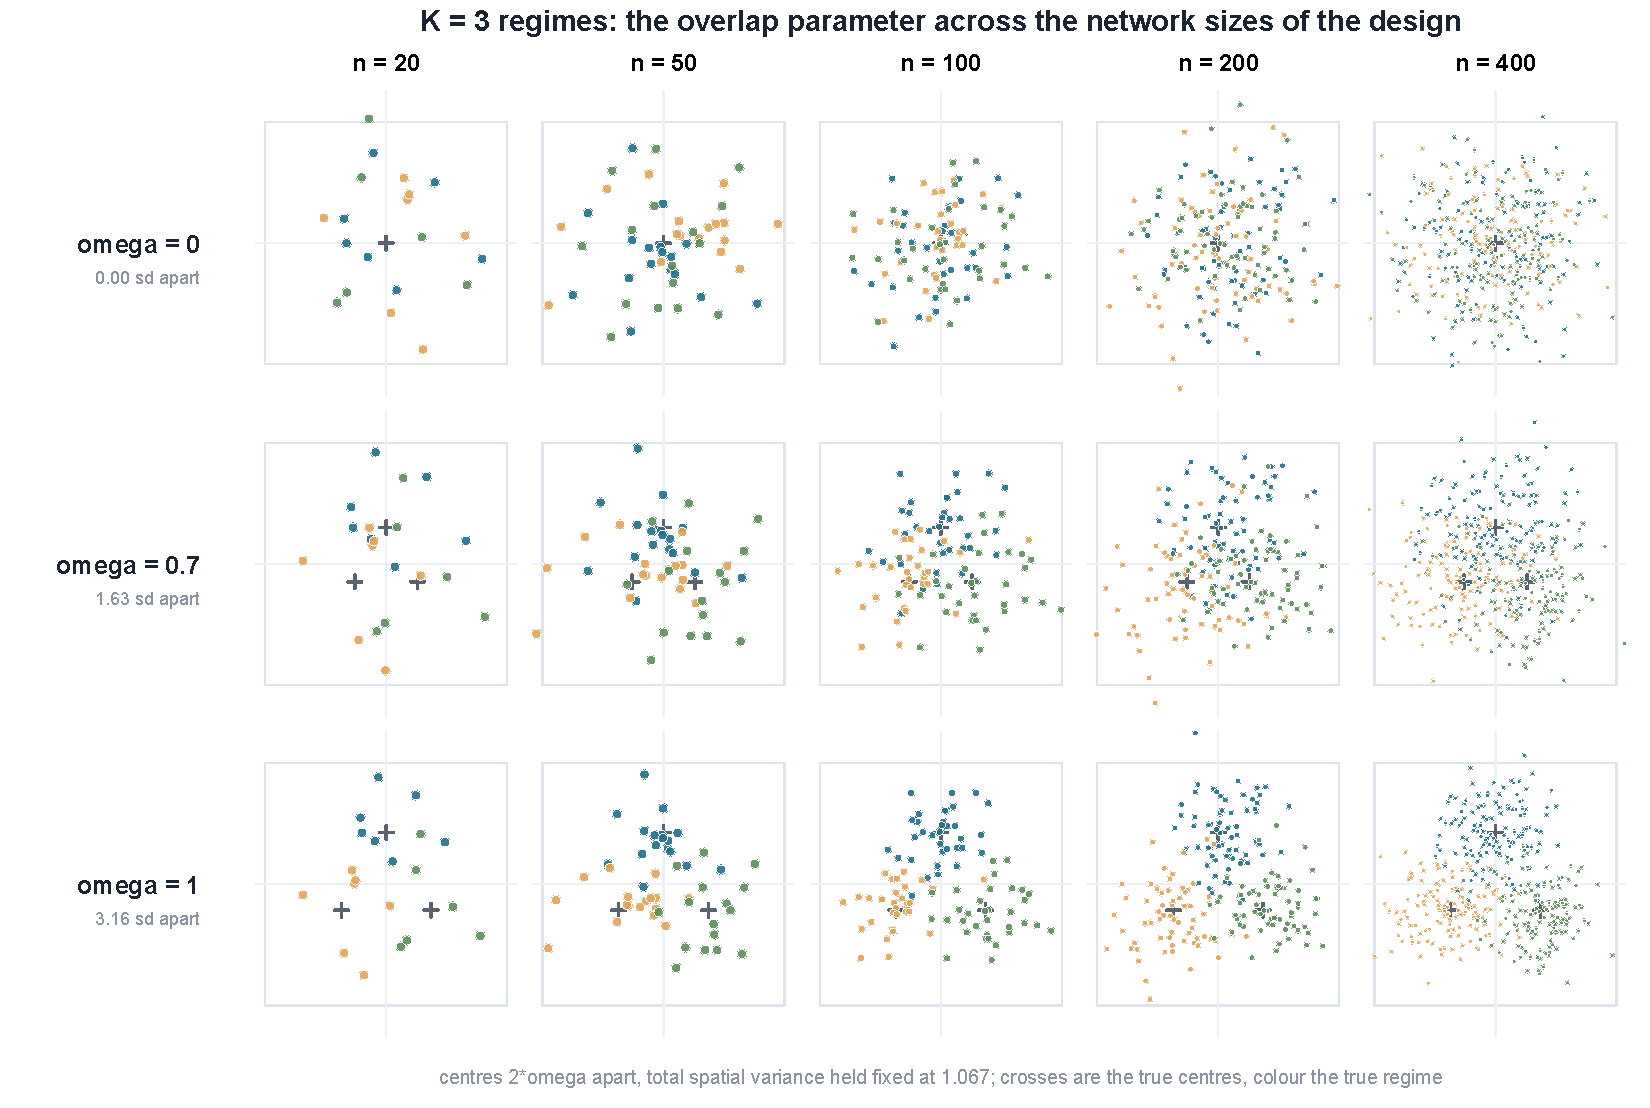
\includegraphics[width=\textwidth]{Figures/fig_design_omega}
\caption{The spatial configuration at $K=3$, for the three levels of the overlap (rows) and the five network sizes (columns). Colour is the true regime, crosses are the centres, and the axes are the same in every panel. The total spatial variance is held at $\nu_{\mathrm{tot}}$ by \eqref{eq:nutot}, so the cloud covers the same area in all fifteen panels and only the separation changes down the rows.}
\label{fig:overlap}
\end{figure}

\subsubsection{The generator}\label{sec3:generator}

Write $I_g = \{i : g_i = g\}$ for the index set of regime $g$ and $n_g = |I_g|$, and $h_{ij}$ for the Euclidean distance between $s_i$ and $s_j$. Spatial correlations are exponential and are parameterised by their \emph{practical range} $R$, the distance at which the correlation falls to $5\%$, so that $e^{-\theta h}$ with $\theta = 3/R$. A replication is generated as follows.

\paragraph{Regime sizes.} $n_1,\dots,n_K$ are equal up to the remainder in the balanced version of the design and proportional to $1:2:\cdots:K$ in the unbalanced one, in both cases subject to a lower bound $n_{\min}$ that guarantees every regime can support its own fit. Labels are assigned in blocks, so that the partition is fixed within a design cell and only the coordinates are random.

\paragraph{Covariate.} One standardised exogenous covariate, an autoregression in time whose innovations are a spatially correlated field:
\begin{equation}
  x_1 = w_1, \qquad
  x_t = a\,x_{t-1} + \sqrt{1-a^2}\,w_t, \qquad
  w_t \sim N_n(0, C_x), \quad (C_x)_{ij} = e^{-3 h_{ij}/R_x},
  \label{eq:dgpcov}
\end{equation}
with $a = 0.7$, so that a shock to the covariate halves in about two periods, and a practical range $R_x = 4$, the whole network, centred and scaled over all $nT$ values. The covariate thus plays the part of a large-scale driver, smoother in space than the error field of the regimes. The two knobs matter: a covariate independent across stations would make a contrast in $\beta$ trivially visible, and a perfectly common one would make it indistinguishable from the latent process. This sits between the two.

\paragraph{Latent processes.} One autoregression per regime, with cross-correlated innovations:
\begin{equation}
  y_t = \mathrm{diag}(G_1,\dots,G_K)\,y_{t-1} + \eta_t,
  \qquad \eta_t \sim N_K(0, \Sigma_\eta),
  \qquad \Sigma_\eta = \Delta R_\rho \Delta,
  \label{eq:dgplatent}
\end{equation}
where $\Delta = \mathrm{diag}(\sigma_{\eta,1},\dots,\sigma_{\eta,K})$, $(R_\rho)_{gh} = \rho$ for $g \neq h$ and $1$ otherwise, $\sigma^2_{\eta,g} = \bar v_y (1-G_g^2)$ and $y_1 \sim N_K(0, \bar v_y R_\rho)$. Tying the innovation variance to $G_g$ holds the stationary variance of every latent process at $\bar v_y$, so that a scenario separating the regimes on their persistence separates them on persistence alone and not on the amplitude of the signal.

The cross-correlation $\rho$ is the central device of the design and is discussed in Section~\ref{sec3:coupling}.

\paragraph{Measurement error.} When all regimes share $(\sigma^2_\epsilon, \sigma^2_\omega, \theta)$ the error is drawn as one global spatial field,
\begin{equation}
  e_t \sim N_n(0, \Sigma), \qquad
  \Sigma = \sigma^2_\epsilon I_n + \sigma^2_\omega \exp(-\theta h),
  \label{eq:dgperr}
\end{equation}
independently over $t$; otherwise one field per regime, independent across regimes,
\begin{equation}
  e_{t,I_g} \sim N_{n_g}(0, \Sigma_g), \qquad
  \Sigma_g = \sigma^2_{\epsilon g} I_{n_g}
           + \sigma^2_{\omega g} \exp(-\theta_g h_{I_g I_g}).
  \label{eq:dgperrg}
\end{equation}
The distinction is deliberate: a block structure in the residual covariance is an intrinsic feature of a scenario in which the regimes differ in their covariance, and an artefact of the generator in one in which they do not. The artefact is not small. A field drawn regime by regime makes the regimes independent of one another, which is what the fitted model assumes and a single field over the network is not, so the break in the correlation at the boundaries reveals the partition by itself, with no parameter differing at all. The scenario S0b of Section~\ref{sec3:scenarios} measures how much it reveals, and with it the information that the scenarios separating the regimes in their covariance receive for free.

\paragraph{Response.} Finally,
\begin{equation}
  z_{ti} = \beta_{0,g_i} + \beta_{1,g_i}\,x_{ti} + y_{t,g_i} + e_{ti},
  \label{eq:dgpz}
\end{equation}
which is the measurement equation \eqref{eq:scmeas} with $K_g = \mathbf{1}_{n_g}$, that is exactly the model the procedure fits. The pseudocode is given in Section~S5 of the Supplementary Material.

\paragraph{The baseline regime.} Every scenario starts from the same regime, whose values are chosen to be generic and readable rather than calibrated. The response is standardised, with unit variance at a location, and that variance is split into the four sources of Table~\ref{tab:baseline}: a covariate and a common dynamics that together explain $60\%$ of it, and a spatially structured and a purely local component that make up the remaining $40\%$. The residual standard deviation is therefore $\sigma = \sqrt{0.40} = 0.63$, the unit in which contrasts in the coefficients are expressed. The mean is $\beta_0 = 2$, two standard deviations above zero: a coefficient of variation of $0.5$, the profile of a positive quantity such as a concentration or a price, which the process rarely takes below zero.

\begin{table}[t]
\centering
\caption{The baseline regime. The variance of the response at a location is $1$; the shares are the part of it each source accounts for.}
\label{tab:baseline}
{\small
\begin{tabular}{llll}
\toprule
source & share & parameter & reading \\
\midrule
covariate & $30\%$ & $\beta_1 = \sqrt{0.30} = 0.55$ & a driver of the process, standardised \\
common dynamics & $30\%$ & $\bar v_y = 0.30$, $G = 0.8$ & a shared temporal signal; a shock halves in $3.1$ periods \\
spatial field & $20\%$ & $\sigma^2_\omega = 0.20$, $R = 2$ & correlated local variation, vanishing at half the network \\
nugget & $20\%$ & $\sigma^2_\epsilon = 0.20$ & measurement error and micro-scale variation \\
\midrule
level & & $\beta_0 = 2$ & a coefficient of variation of $0.5$ \\
\bottomrule
\end{tabular}}
\end{table}

\subsubsection{Coupling of the latent processes}\label{sec3:coupling}

An earlier version of this design generated each regime by simulating the model on its own sub-network, which is what the specification literally says: regime $g$ has its own latent process and two locations in different regimes are uncorrelated. That is faithful and it is also useless as an experiment. It makes the partition identifiable from the correlation structure alone, whatever the parameters: generating with \emph{identical} parameters in the two regimes and one latent path per regime recovers the true partition in every replication, while generating the same data with one shared latent path gives an Adjusted Rand Index of $0.14$. What such a design measures is the recovery of the latent split, not of any difference in $\Psi_g$, so a scenario separating the regimes only in the dynamics or only in the spatial covariance would be testing nothing of the sort.

The coupling is therefore made an explicit factor through $\rho$ in \eqref{eq:dgplatent}. At $\rho = 1$ the regimes share their dynamics and the partition can be found \emph{only} through the parameters, which is the honest and hard case and the one used throughout. At $\rho = 0$ the processes are independent, which is the model-consistent and easy case, retained as a single reference cell so that the size of the confound can be read off directly.

One consequence deserves stating. With equal transition coefficients the correlation of the latent processes is exactly $\rho$; with different ones it is
\begin{equation}
  \mathrm{Cor}(y_{t,g}, y_{t,h}) =
  \rho\,\frac{\sqrt{(1-G_g^2)(1-G_h^2)}}{1 - G_g G_h} \;<\; 1
  \qquad \text{whenever } G_g \neq G_h ,
  \label{eq:leak}
\end{equation}
however large $\rho$ is. Two autoregressions with different persistence cannot be perfectly correlated, so a scenario that separates the regimes on their dynamics necessarily leaks a little information through the latent paths. The design measures that leak instead of concealing it.

\subsubsection{Scenarios: what separates the regimes}\label{sec3:scenarios}

The parametric channel is organised around \emph{which component of $\Psi_g$ separates the regimes}, and by how much. Regime $1$ always carries the baseline of Table~\ref{tab:baseline}; regime $K$ carries the full contrast; with $K=3$ the middle regime sits halfway, so that $K=2$ and $K=3$ mean the same thing by the same numbers. Contrasts come at up to three levels, weak, medium and strong. With $K=1$ every scenario collapses to the baseline. Each scenario opens one route by which the data can reveal the regimes and keeps the others closed, so that each answers one question:

\begin{description}[leftmargin=1.2em,itemsep=3pt,topsep=3pt]
  \item[\textbf{S0 --- no separation.}] Every regime carries the baseline, the latent path is shared and one error field spans the network, so the distribution of the data does not depend on the partition. \emph{Does the procedure invent regimes?} It measures the false positives of the selection rule and the compactness the penalty manufactures on its own.
  \item[\textbf{S0b --- no separation, error field by regime.}] As S0, but with the error field drawn regime by regime. No parameter differs, so whatever is recovered comes from the independence of the regimes alone. \emph{How much does the block structure of the field reveal by itself?} This is the information that S3, S4 and S5 receive for free, and S0b is the baseline against which their recovery is read.
  \item[\textbf{S1 --- separation in the regression coefficients.}] The regimes share the dynamics and the covariance and differ only in the effect of the covariate, which in the last regime is $1.25$, $1.5$ or $2$ times the baseline ($0.22$, $0.43$ and $0.87$ residual standard deviations). \emph{Are regimes found when the driver acts with a different strength?} This is the design under which the cross-sectional intuition applies most directly.
  \item[\textbf{S2 --- separation in the latent dynamics.}] The regimes share $\beta$ and the covariance and differ in the persistence $G_g$: $0.7$ or $0.2$ against $0.8$, that is shocks that halve in $1.9$ or $0.4$ periods against $3.1$. \emph{Are regimes with slow and fast dynamics told apart?} It tests whether the assignment score \eqref{eq:score}, which sees the dynamics only through the smoothed state, can discriminate regimes that differ in nothing else.
  \item[\textbf{S3 --- separation in the spatial covariance.}] The regimes share $\beta$ and the dynamics and differ in how the residual variance is organised in space: in the last regime the practical range falls from $2$ to $1$ or $0.25$ and the nugget share rises from $0.5$ to $0.6$ or $0.8$, the total staying the same --- a regime dominated by micro-scale variation, as sites exposed to local sources are against background ones. \emph{Are regimes found that differ only in their spatial texture?} This is the hardest case for the assignment score, which retains only the total variance $\sigma^2_{\epsilon g} + \sigma^2_{\omega g}$ and is blind to any reallocation between the two components leaving their sum unchanged; the scenario documents that limitation and measures how much of the separation the parameter step recovers through the exact likelihood.
  \item[\textbf{S4 --- joint separation.}] All three components differ, at the medium level. \emph{Does the procedure work in the case it is built for?} This is the scenario closest to the intended use of the model and the one of the reference cell.
  \item[\textbf{S5 --- reference.}] As S4, but with $\rho = 0$ and the error field drawn regime by regime, reproducing the model-consistent generator discussed in Section~\ref{sec3:coupling}. \emph{How much easier is the problem when the data follow the model exactly?} Its distance from S4 is the size of the confound.
\end{description}

Table~\ref{tab:dgp} gives the parameter values each scenario sets, regime by regime.

\begin{table}[t]
\centering
\caption{The scenarios side by side, at $K = 3$. A parameter that differs between the regimes is printed in bold as its values in regimes 1 / 2 / 3; one printed once is common to all of them. Regime 1 always carries the baseline of Table~\ref{tab:baseline}: $\beta = (2, 0.55)$, $\sigma^2_\epsilon = \sigma^2_\omega = 0.20$ (a nugget share of $0.5$), a practical range of $2$, $G = 0.8$ and a stationary latent variance of $0.30$, so a residual standard deviation of $\sigma = 0.63$; the total residual variance $\sigma^2_\epsilon + \sigma^2_\omega$ is the same in every regime. $\Delta\beta_1/\sigma$ is the contrast between regimes 1 and 3 in units of $\sigma$. $\rho$ is the correlation of the innovations of the latent processes \eqref{eq:dgplatent}, and the error field is drawn once over the whole network \eqref{eq:dgperr} or regime by regime \eqref{eq:dgperrg}.}
\label{tab:dgp}
{\small\setlength{\tabcolsep}{4pt}\begin{tabular}{llllllrrl}
\toprule
& & \multicolumn{5}{c}{regime parameters, regimes 1 / 2 / 3} & & \\
\cmidrule(lr){3-7}
id & differs in & $\beta_1$ & $\Delta\beta_1/\sigma$ & $G$ & nugget share & practical range & $\rho$ & error field \\
\midrule
S0 & nothing & 0.55 & 0.00 & 0.80 & 0.50 & 2.00 & 1 & one \\
S0b & nothing & 0.55 & 0.00 & 0.80 & 0.50 & 2.00 & 1 & by regime \\
S1a & $\beta_1$ & \textbf{0.55 / 0.62 / 0.68} & 0.22 & 0.80 & 0.50 & 2.00 & 1 & one \\
S1b & $\beta_1$ & \textbf{0.55 / 0.68 / 0.82} & 0.43 & 0.80 & 0.50 & 2.00 & 1 & one \\
S1c & $\beta_1$ & \textbf{0.55 / 0.82 / 1.10} & 0.87 & 0.80 & 0.50 & 2.00 & 1 & one \\
S2a & $G$ & 0.55 & 0.00 & \textbf{0.80 / 0.75 / 0.70} & 0.50 & 2.00 & 1 & one \\
S2b & $G$ & 0.55 & 0.00 & \textbf{0.80 / 0.50 / 0.20} & 0.50 & 2.00 & 1 & one \\
S3a & covariance & 0.55 & 0.00 & 0.80 & \textbf{0.50 / 0.55 / 0.60} & \textbf{2.00 / 1.50 / 1.00} & 1 & by regime \\
S3b & covariance & 0.55 & 0.00 & 0.80 & \textbf{0.50 / 0.65 / 0.80} & \textbf{2.00 / 1.12 / 0.25} & 1 & by regime \\
S4 & all three & \textbf{0.55 / 0.68 / 0.82} & 0.43 & \textbf{0.80 / 0.65 / 0.50} & \textbf{0.50 / 0.60 / 0.70} & \textbf{2.00 / 1.25 / 0.50} & 1 & by regime \\
S5 & all three & \textbf{0.55 / 0.68 / 0.82} & 0.43 & \textbf{0.80 / 0.65 / 0.50} & \textbf{0.50 / 0.60 / 0.70} & \textbf{2.00 / 1.25 / 0.50} & 0 & by regime \\
\bottomrule
\end{tabular}
}
\end{table}

\begin{figure}[t]
\centering
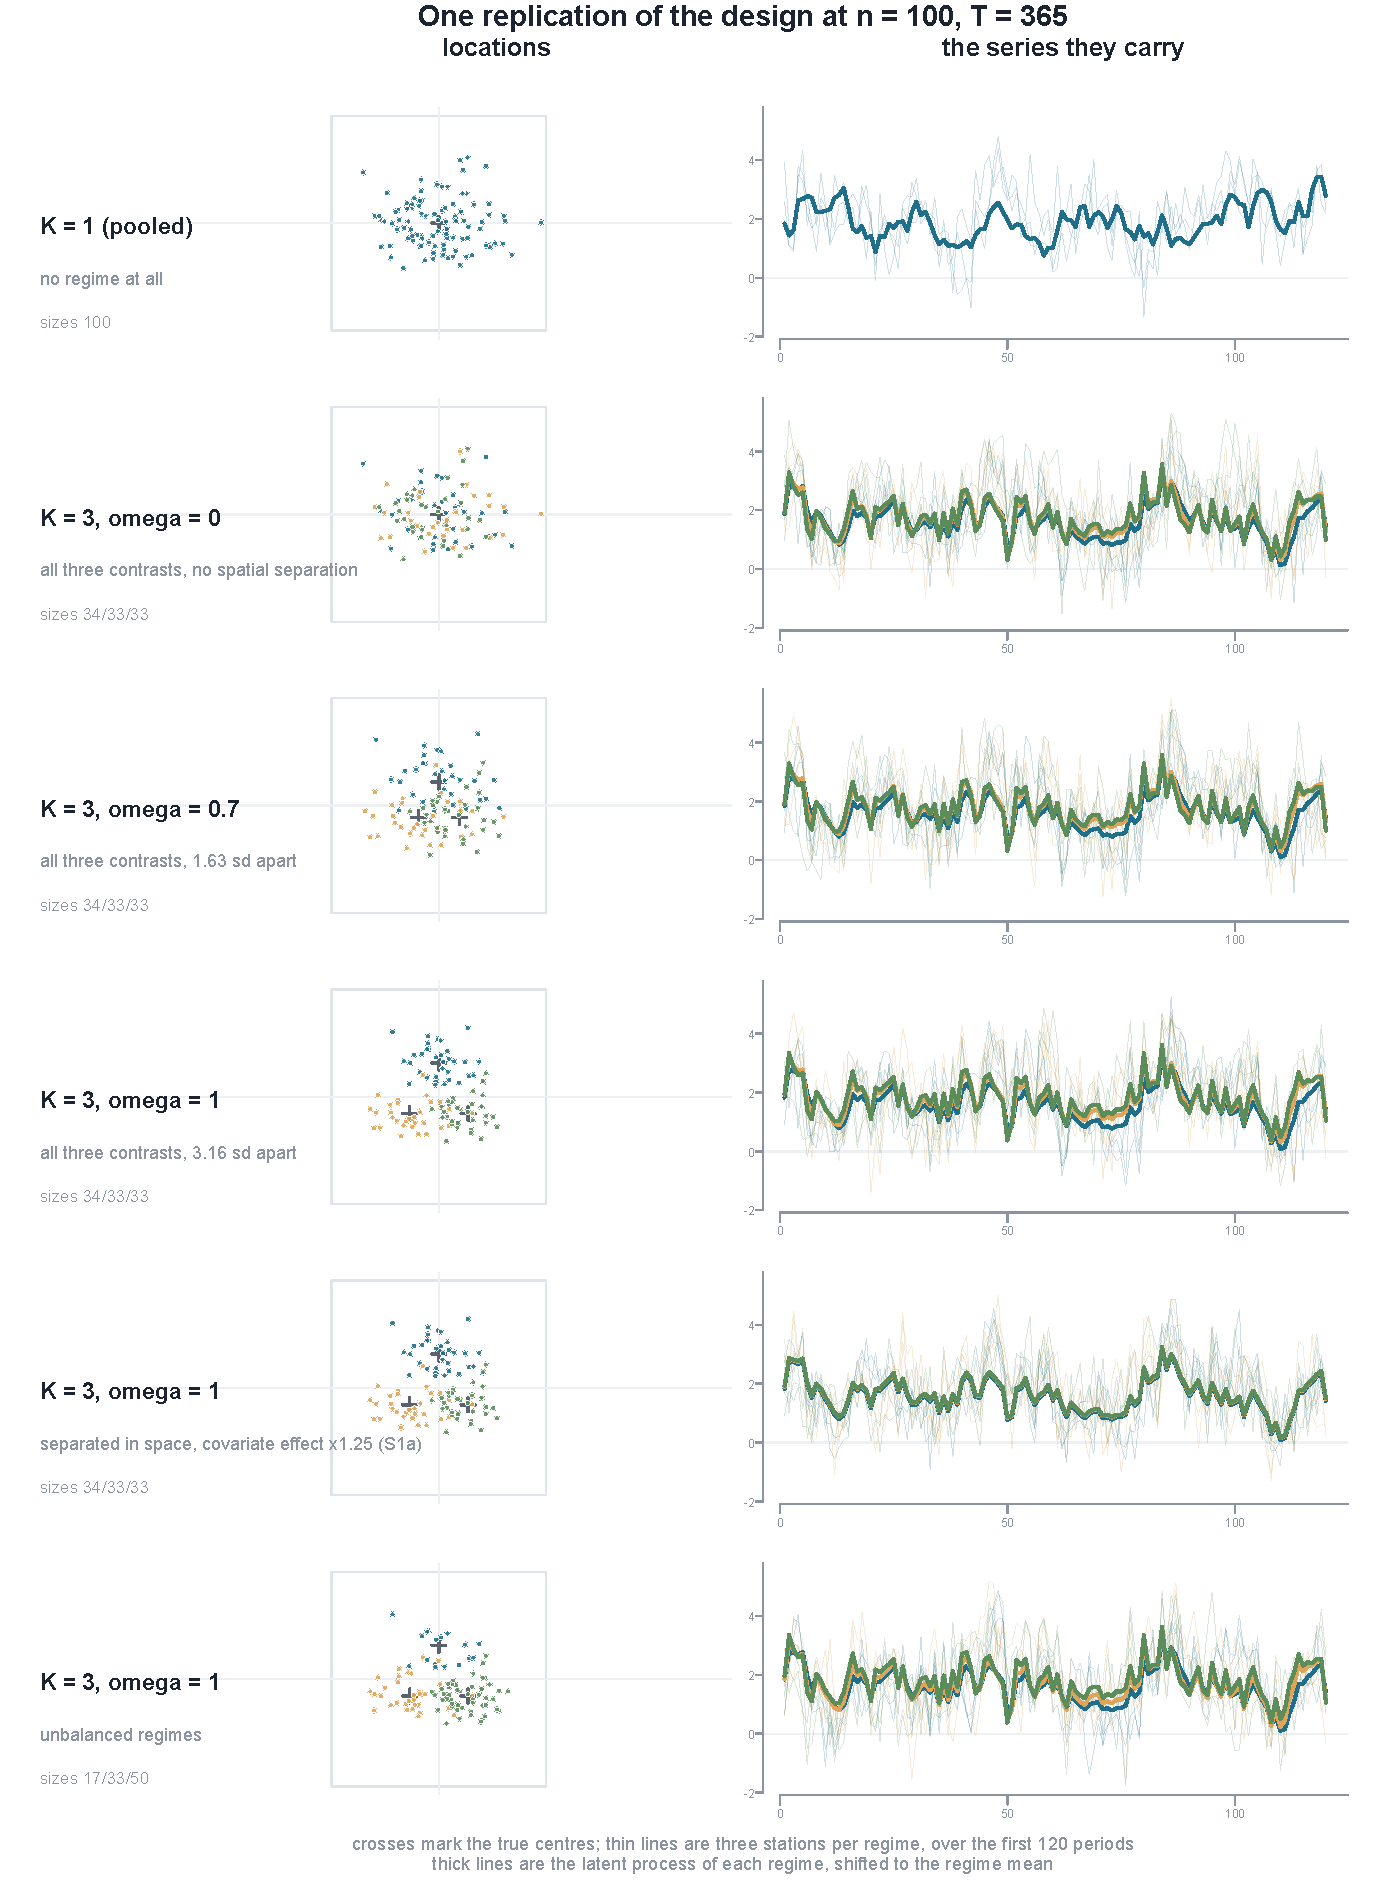
\includegraphics[width=\textwidth]{Figures/fig_dgp_examples}
\caption{One replication of the design at the reference network size $n = 100$ and at $T = 365$, for six combinations of the number of regimes, the overlap and the scenario. Left: the locations, coloured by true regime, crosses at the cluster centres. Right: the series they carry over the first $120$ periods --- three stations per regime in thin lines, the latent process of each regime, shifted to the regime mean, in thick lines. Rows two to four raise the overlap at a fixed scenario; row five holds the overlap at its largest and weakens the parametric contrast instead, which is the case the design exists to separate.}
\label{fig:dgp}
\end{figure}

\subsubsection{The neighbourhood graph, and why it is a factor}\label{sec3:graph}

Section~\ref{sec2:potts} argues why a Potts penalty belongs on point-referenced data and what it takes to use it there. Two of its points are properties of the design. The number of neighbours $m$ of the graph is a choice of the analyst and not a feature of the problem, so it is a factor of the experiment rather than a fixed setting, with levels $\{3, 5, 10\}$. And the graph is built with the metric of the covariance. In the design the plane is Euclidean and the question does not arise, but on geographic coordinates it does: on a network of $300$ locations spread over a regional box at $45^\circ$ of latitude, at $m=5$, a graph built on raw longitude and latitude shares only $78.5\%$ of its edges with the geodesic one, and $40.8\%$ of its edges are more east-west than north-south against $50.9\%$ for the correct metric. The third point, that spatial proximity enters the model twice, is what the cells at $\omega = 0$ and the scenario S0 measure: when the data carry no regimes the penalty is the only term of the objective that prefers one partition to another, so a procedure that returns a spatially compact partition there is reporting the penalty and not the data.

The quantity that governs how much the penalty can help is not the density of the graph but the share of its edges that join two \emph{different} true regimes: those are precisely the pairs the penalty rewards for agreeing when they should not. For $K$ balanced regimes a graph carrying no information about the partition has a crossing share of $1 - 1/K$. Measured at $K=3$ over the design, that share is $0.68$ at $\omega=0$ --- the value of an uninformative graph, to two decimals --- $0.41$ at $\omega=0.70$ and $0.13$ at $\omega=1$, and it is remarkably insensitive to $k$: from $n = 100$ on, the three values of $k$ reproduce it to within $0.03$. What $k$ does change is the number of edges, from a mean degree of $3.8$ at $k=3$ to $12.5$ at $k=10$. Under a fixed scale of the penalty that would multiply the weight it carries at a given $\phi$; under the default scale of Section~\ref{sec:phiscale} it does not, since $c$ divides by the mean degree. The number of neighbours spreads the same pull over more and longer edges, while the information the graph holds about the partition is set by the geometry alone. Figure~\ref{fig:knn} shows the graphs and Figure~\ref{fig:graphnum} the two statements in numbers.

\begin{figure}[t]
\centering
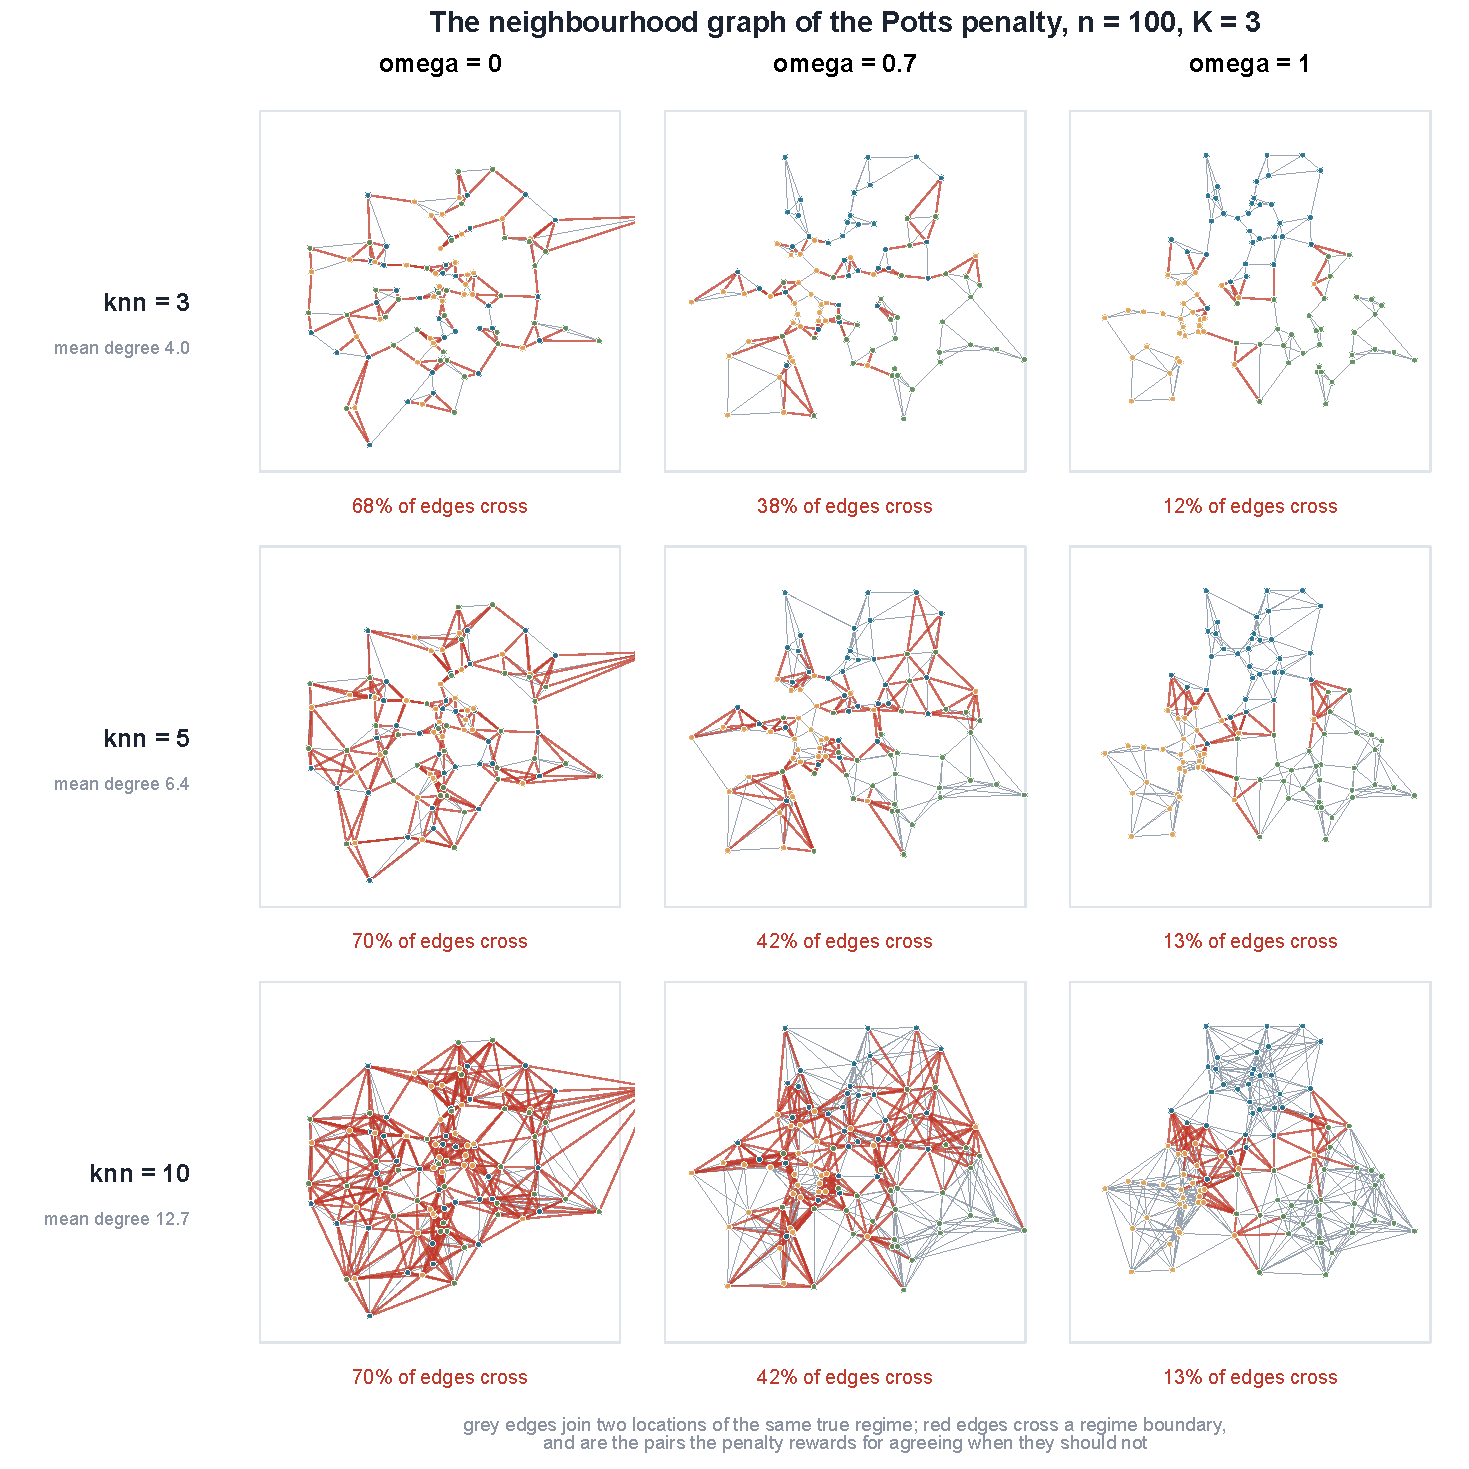
\includegraphics[width=0.92\textwidth]{Figures/fig_design_knn}
\caption{The neighbourhood graph the penalty is evaluated on, at $n=100$ and $K=3$, for the three values of $k$ (rows) and the three levels of the overlap (columns). Grey edges join two locations of the same true regime; red edges cross a regime boundary and are the pairs the penalty rewards for agreeing when they should not. The simulated data are identical across a row: $k$ changes the objective, not the observations.}
\label{fig:knn}
\end{figure}

\begin{figure}[t]
\centering
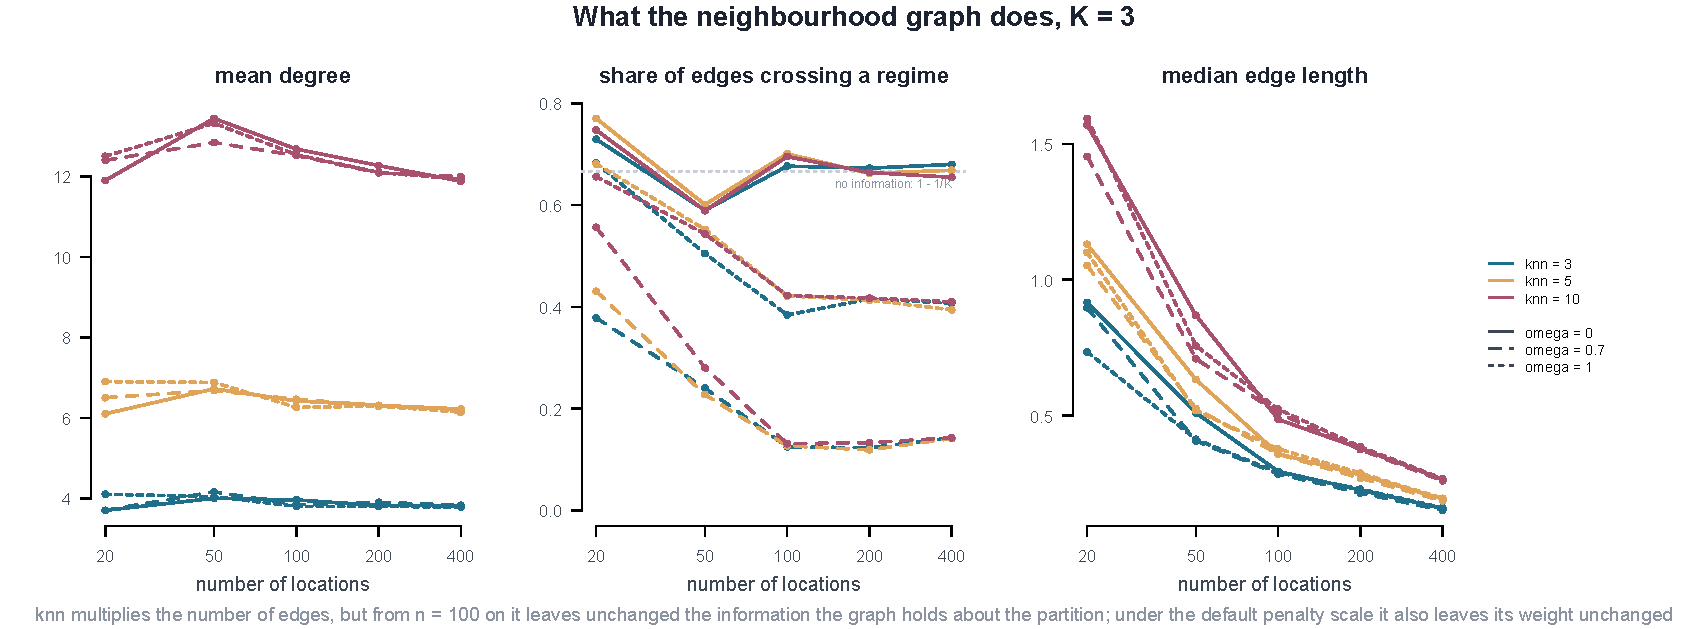
\includegraphics[width=\textwidth]{Figures/fig_design_graph}
\caption{What the neighbourhood graph does, at $K=3$. Left: the mean degree, set by $k$ alone. Centre: the share of edges that cross a true regime boundary, set by the overlap alone from $n=100$ on; the dotted line is $1-1/K$, the value of a graph carrying no information about the partition. Right: the median edge length. Line colour is $k$, line type is the overlap.}
\label{fig:graphnum}
\end{figure}

\subsubsection{Factors and evaluation metrics}\label{sec3:factors}

The factors of the experiment are the number of locations $n \in \{20, 50, 100, 200, 400\}$, from a small network to a large one; the series length $T \in \{60, 120, 365\}$, a short, a medium and a long series, the shortest still spanning about twenty half-lives of a shock at the baseline persistence; the number of regimes $K \in \{1, 3\}$, the first being the null case of Section~\ref{sec3:overlap}; the overlap $\omega \in \{0, 0.70, 1\}$, that is separations of $0$, $1.63$ and $3.16$ standard deviations; the neighbourhood size $k \in \{3, 5, 10\}$ of Section~\ref{sec3:graph}; the balance of the regime sizes, equal or proportional to $1:2:\cdots:K$; and the eleven scenarios of Table~\ref{tab:dgp}. The procedure is fitted over a grid of $k \in \{1,\dots,4\}$ regimes and penalties $\phi \in \{0, 0.5, 1\}$, so that the model-selection behaviour is assessed jointly with the estimation behaviour, and the recovery of the parameters is read at the true number of regimes and $\phi = 0.5$. The estimator is held to the same floor as the generator: a configuration that would leave a regime with fewer than $n_{\min} = 6$ locations is not fitted, since on fewer locations the range of the regime is not identified, and the grid simply omits it. At $n = 20$ this removes $k = 4$. The floor is not only a matter of principle: below it the fit is also ruinously slow, a $k=4$ fit on twenty locations taking minutes where $k=3$ takes a second.

\paragraph{The design is not a full factorial.} Crossing every factor with every other is $2970$ cells at $K=3$ alone, most of them answering no question. The experiment is instead a factorial in the three factors that interact --- how many locations, how separated the regimes, how long the series --- together with one-factor-at-a-time margins around a reference cell for the factors that are there to establish that the results do not turn on them. The reference cell is $n = 100$, $T = 120$, $K = 3$, $\omega = 0.70$, balanced, scenario S4, $k = 5$. Five blocks result:

\begin{description}[leftmargin=1.2em,itemsep=3pt,topsep=3pt]
  \item[\textbf{Core} (45 cells).] $n \times \omega \times T$ fully crossed at the reference scenario and graph: recovery as a function of the three quantities that govern it.
  \item[\textbf{Null} (15 cells).] The same $n \times T$ grid at $K=1$, where there is no regime to find and the question is whether the procedure invents one.
  \item[\textbf{Scenarios} (165 cells).] All eleven scenarios crossed with $n$ and $\omega$ at the reference $T$: what has to differ between regimes for the difference to be found.
  \item[\textbf{Graph} (45 cells).] $k$ crossed with $n$ and $\omega$, the two factors it interacts with, a dense graph on a small network behaving unlike a sparse one on a large network.
  \item[\textbf{Balance} (15 cells).] Unequal regime sizes crossed with $n$ and $\omega$.
\end{description}

The blocks overlap on the reference configuration and are deduplicated, leaving $255$ cells, of which $252$ admit the requested imbalance with regimes of at least $n_{\min}$ locations. Each is replicated $M = 100$ times from a seed derived from the replication index, so that a cell is reproducible on its own and the same replication carries the same geometry across scenarios.

\paragraph{Evaluation metrics.} Performance is measured along four dimensions:
\begin{enumerate}[leftmargin=*,itemsep=2pt,topsep=3pt]
  \item \emph{Recovery of the partition}, by the Adjusted Rand Index \citep{HubertArabie1985} between the estimated and the true partition, computed at the true number of regimes and at the selected one. The index is invariant to relabelling; the share of correctly assigned locations, which is not, is also reported after aligning the estimated labels to the true ones by the majority rule.
  \item \emph{Accuracy of the regime-specific parameters}, by the bias and the root mean squared error of the components of $\Psi_g$ over replications, after the same alignment. These are Monte Carlo summaries and not quantities a single replication could produce, so the record kept is one row per replication, regime and parameter, holding the truth beside the estimate.
  \item \emph{Predictive accuracy}, measured against the conditional mean and not against the response. The target is
  \begin{equation}
    \mu_{ti} = x_{ti}' \beta_{g_i} + K_i\, y_{t,g_i} ,
    \label{eq:signal}
  \end{equation}
  the systematic part of \eqref{eq:dgpz}, because the measurement error in $z$ is irreducible and scoring against $z$ would add the same constant to every model and compress every comparison towards one. The estimate is the fitted signal $\hat\mu_{ti} = x_{ti}' \hat\beta_{\hat g_i} + K_i \hat y_{t,\hat g_i}$, not the conditional expectation of $z$ given what was observed: on a complete record the latter returns the data itself and measures nothing. Errors are reported relative to the pooled STEM fit, so the gain attributable to the regimes is immediately readable.
  \item \emph{Model selection}, by the frequency with which the two-step rule of Section~\ref{sec:tuning} recovers the true number of regimes, and by the behaviour of the information criteria across the penalty grid. The pooled model competes with the clustered configurations inside the rule and is returned when no partition improves on it, so the cells $K = 1$ measure directly how often a homogeneous network is split.
\end{enumerate}

\paragraph{The station is the unit of the error measures.} With point-referenced data the unit that carries a regime is the location, so the error that answers ``does the clustering help, and where'' is computed within a station over time and then examined across stations. The pooled root mean squared error over all $nT$ cells is, on a balanced panel, exactly the root mean of the per-station mean squared errors,
\begin{equation}
  \mathrm{RMSE}_{\mathrm{pool}}
  = \sqrt{\frac{1}{nT}\sum_{i=1}^{n}\sum_{t=1}^{T} (\hat\mu_{ti} - \mu_{ti})^2}
  = \sqrt{\frac{1}{n}\sum_{i=1}^{n} \mathrm{MSE}_i} ,
  \label{eq:pooledrmse}
\end{equation}
so it is a summary \emph{of} the per-station measure rather than an alternative to it, and it destroys the distribution across stations that shows the regimes at work. On an unbalanced panel it is not even that, since it then weights a station by how many periods it was observed. Both are recorded and the per-station file is what the tables are built from. On real data the conditional mean is not available and the honest measure is out-of-sample against $z$ with spatio-temporal blocking, which is a different exercise.

In every case the pooled STEM model is retained as the benchmark: the question the experiments answer is not whether SC-STEM fits better --- a model with $k$ times as many parameters generally will --- but whether it recovers the regimes that generated the data, and whether the additional parameters buy predictive accuracy that the pooled model does not deliver.

\paragraph{What is recorded.} Each replication writes four records sharing the primary key (cell, replication): one row per replication with the selected configuration, the recovery indices, the errors and the wall time; one row per replication, regime and parameter with truth beside estimate; one row per replication and station with its coordinates, its true and estimated regime and its errors over time; and, for the first five replications of each cell, one row per station and period with the covariate, the response, the true conditional mean, the labels and the fitted signals of the clustered and of the pooled model. The last is $nT$ rows and is kept only for the representative-replication figures. The four join on the key and on nothing else; the factors are carried beside it for filtering, the overlap being a double that no join should rest on.

\subsection{Results}\label{sec3:results}

\TODO{The simulation study has been designed but not yet executed. This subsection will report, for each design and each separation level: the ARI distribution across replications and penalties, the bias and RMSE of the regime-specific parameters, the relative predictive accuracy against the pooled fit, and the selection frequencies of the two-step rule. The per-design tables and the representative replications go to the supplementary material.}

%%%%%%%%%%%%%%%%%%%%%%%%%%%%%%%%%%%%%%%%%%%%%%%%%%%%%%%%%%%%%%%%%%%%%%%%%%%%%%%
\section{Computational and inferential aspects}\label{sec:compinf}
%%%%%%%%%%%%%%%%%%%%%%%%%%%%%%%%%%%%%%%%%%%%%%%%%%%%%%%%%%%%%%%%%%%%%%%%%%%%%%%

This section collects the implementation choices that complete Algorithm~\ref{alg:scstem}, together with the two properties --- non-monotonicity and degeneracy --- that the transfer of the spatially-clustered apparatus to a spatio-temporal model brings with it.

\subsection{Algorithmic details}\label{sec:algdetails}

\paragraph{Initialization.} The initial partition is obtained by $k$-means on the location-wise averages of the covariates, standardized and compressed by principal components retaining $90\%$ of the cumulative variance, with multiple random restarts and an admissibility filter that discards starting partitions whose smallest regime could not support a cluster-wise fit. For intercept-only specifications, where the covariate means carry no information, the spatial coordinates are used instead. Initializing on the covariates rather than on the coordinates leaves spatial contiguity entirely to the Potts penalty, so that $\phi$ can be read as the price paid for spatial coherence rather than as a constraint built into the starting point. Any externally computed partition can be supplied in place of this default.

\paragraph{Empty and undersized regimes.} Along the iterations a regime can shrink below the number of locations required to estimate its parameters. Rather than aborting, the implementation freezes such a regime at its last valid parameter values and keeps it available to the assignment step, so that locations can flow back into it; a regime that never obtained a valid fit is excluded from the assignment altogether. A configuration whose final partition still contains empty or undersized regimes is flagged as inadmissible and excluded from model selection, since its likelihood is not comparable with that of a configuration with $k$ genuine regimes.

\paragraph{Final refit.} On convergence the regimes are re-estimated once on the best partition visited, holding the labels fixed. All reported coefficients, variance components and information criteria come from this refit and are based on the \emph{exact} cluster-wise log-likelihoods returned by the EM algorithm, not on the pseudo-likelihood \eqref{eq:score} used to rank regimes during the assignment step. The number of free parameters of a configuration is
\begin{equation}\label{eq:npar}
  \mathcal{K} \;=\; k_{\mathrm{eff}} \left(r + 3 + 3p\right),
\end{equation}
for a diagonal specification of $G$ and $\Sigma_\eta$ with $r$ covariates and latent dimension $p$, where $k_{\mathrm{eff}}$ counts the regimes that could actually be re-estimated: $r$ regression coefficients, the three parameters $(\sigma^2_\epsilon, \sigma^2_\omega, \theta)$ of the measurement covariance, and $p$ parameters each for $G$, $\Sigma_\eta$ and $m_0$.

\paragraph{Computational cost.} Each parameter step runs $k$ independent EM algorithms, one per regime, and the regimes are trivially parallelizable. Within a regime of size $d_k$, the dominant cost is the factorization of the $d_k \times d_k$ measurement covariance at each EM iteration, that is $O(d_k^3)$, so that partitioning the network is computationally advantageous relative to the pooled fit whenever the regimes are of comparable size: $\sum_k d_k^3 \ll d^3$ for any non-trivial partition. The label step is a single sweep over the $d$ locations with cost $O(d\, k\, \bar{m})$, where $\bar{m}$ is the average number of neighbors, and the score matrix \eqref{eq:score} costs $O(d\, k\, T)$.

\subsection{Degeneracy, the minimum-size constraint and the swap pass}\label{sec:degeneracy}

Within-cluster homogeneity is exactly what the assignment step pursues, and this creates a degeneracy that has to be controlled. As locations are reallocated to the regime that fits them best, the residual variability within each regime falls, and with it the estimated variance components $\sigma^2_{\epsilon k}$ and $\sigma^2_{\omega k}$. But the score \eqref{eq:score} rewards a small $v_k$: for a location whose residuals under two regimes are comparable, the regime with the smaller total variance wins. Left unconstrained, the process is self-reinforcing --- the regime with the smallest residual variance attracts locations, which makes it more homogeneous, which lowers its variance further --- and the partition collapses onto a single regime. This is the clusterwise counterpart of the degenerate-likelihood problem of Gaussian mixtures, where a component can concentrate on a few observations and drive its variance to zero. We observed the collapse empirically even at $\phi = 0$, that is with no spatial forcing at all, which confirms that it originates in the likelihood and not in the penalty.

The control is a constraint on the size of the regimes. A location may leave its current regime only if that regime remains at or above a minimum size $n_{\min}$, set by default to the number of parameters required by a cluster-wise fit. The constraint acts on the feasible set rather than on the objective: every configuration visited by the algorithm is admissible by construction, and the monotonicity of the ICM sweep is preserved within the feasible set, since each label still maximizes its own penalized contribution over the labels that remain available to it.

The constraint has a cost of its own, and it is severe on small networks. A location sitting in a regime that is exactly at the minimum size can never move, whatever its fit, because moving it would violate feasibility. With $d$ small relative to $k \cdot n_{\min}$, a large share of the partition can therefore stay frozen at its initial value, and the algorithm reports convergence on a configuration it was never free to leave. The remedy is to add a class of moves that the constraint cannot block. Each sweep is followed by a \emph{size-preserving swap pass}: the labels of two locations belonging to different regimes are exchanged whenever the exchange strictly increases $Q$. A swap leaves every regime size unchanged, so feasibility holds automatically, and it is accepted only on strict improvement, so the monotonicity of the sweep is preserved. Swaps let the algorithm explore configurations that the constraint makes unreachable through single moves, and in practice they are what allows a well-separated partition to be recovered on a small network.

Evaluating every candidate swap is quadratic in $d$, which would dominate the cost of a sweep. The implementation therefore vectorizes the pass over pairs and prunes it with an exact upper bound on the gain achievable by any swap between two given regimes: since exchanging the labels of $i$ and $j$ can alter the penalty only through the edges incident to $i$ and $j$, the penalty gain cannot exceed $\phi c\,(m_i + m_j + 1)$, where $m_i$ is the number of neighbors of location $i$. Pairs whose likelihood gain is below the negative of that bound cannot improve $Q$ and are discarded without further computation. The bound is exact, so the pruning changes the running time and not the result.

\subsection{On monotonicity}\label{sec:monotone}

Each of the two steps of Algorithm~\ref{alg:scstem} is monotone in its own right. The ICM sweep cannot decrease $Q$ at fixed parameters, the swap pass accepts only strict improvements, and the EM algorithm cannot decrease the exact likelihood of a regime at fixed labels. It does not follow that the alternation is monotone, and in general it is not: the trace of the objective may well show a decrease from one iteration to the next.

The reason is structural, and it is the price of Section~\ref{sec2:score}. The label step maximizes the penalized \emph{pseudo}-likelihood \eqref{eq:Q}, built on the conditional scores \eqref{eq:score}; the parameter step maximizes the \emph{exact} within-regime likelihood through the EM algorithm. These are two different functions of the same parameters. They agree on what a good partition looks like --- both reward regimes whose members are well described by common parameters --- but they are not related by an inequality, so an EM update that raises the exact likelihood of a regime can lower the pseudo-likelihood contributions of some of its members, and hence $Q$. Had the exact likelihood factorized across locations, the two objectives would coincide and the usual monotonicity argument would apply; it does not factorize precisely because $\Sigma_{e,k}$ is not diagonal. Non-monotonicity is therefore a property of the spatio-temporal specification, not a defect of the implementation and not a numerical tolerance issue, and it has no counterpart in the cross-sectional models from which the algorithmic apparatus is borrowed.

Three practical consequences follow. First, the algorithm keeps track of the best configuration visited and returns that one, rather than the last: the final refit is performed on the best partition, not on the terminal one. Second, convergence cannot be declared on the basis of a monotone objective, so the stopping rule combines several criteria --- an unchanged partition, an improvement below tolerance, the reappearance of a previously visited partition, which detects cycling, and an iteration budget. Third, the trace of the objective is reported as a diagnostic rather than as a guarantee, and a decreasing trace is informative about the tension between the two objectives rather than a sign of failure.

\subsection{The scale of the spatial penalty}\label{sec:phiscale}

In a cross-sectional spatially-clustered model each unit contributes a single observation to the likelihood, so the differences $\ell_i(k) - \ell_i(k')$ are of order one and a penalty $\phi$ of order one balances fit against cohesion. This is what makes a grid such as $\phi \in [0,1]$ meaningful across applications in that literature. In the spatio-temporal case the same grid means nothing: each location contributes $T$ observations, so the log-likelihood differences grow with the length of the series and with the scale of the response, and a penalty that reorganizes the partition for $T=100$ is invisible for $T=2000$. The factor $c$ in \eqref{eq:Q} restores comparability.

The default is data-driven. Let $\Delta_i = \max_k \ell_i(k) - \min_k \ell_i(k)$ be the spread of the scores of location $i$ across the candidate regimes, that is the likelihood value of choosing the best regime rather than the worst for that location. The scale is set to
\begin{equation}\label{eq:cauto}
  c \;=\; \frac{\mathrm{median}_i\, \Delta_i}{\bar{m}},
\end{equation}
the median spread divided by the average number of neighbors, and it is computed once, at the first sweep, and held fixed thereafter so that the objective does not change between iterations. With this normalization, $\phi = 1$ is the point at which full agreement with one's entire neighborhood is worth about as much as the typical gain from picking the best-fitting regime, so a grid $\phi \in [0,2]$ is informative on any dataset regardless of $T$ and of the units of the response.

\subsection{Missing observations}\label{sec:missing}

Monitoring networks are rarely complete: instruments fail, stations are serviced, and series start and end at different dates. The state-space form accommodates this at almost no cost, and we follow the treatment of \citet[Sections~2.7 and~4.10]{DurbinKoopman2012}.

\paragraph{Filtering and smoothing.} Suppose that at time $t$ only some of the elements of $z_t$ are observed. Let $W_t$ be the selection matrix whose rows are the corresponding rows of the identity, and write $z^*_t = W_t z_t$. The measurement equation \eqref{eq:scmeas} is replaced at that time point by
\begin{equation}\label{eq:selection}
  z^*_t = Z^*_t\, y^{(k)}_t + e^*_t, \qquad
  Z^*_t = W_t Z, \quad e^*_t \sim N\!\left(0,\; W_t \Sigma_{e,k} W_t^\top\right),
\end{equation}
with the regression term selected in the same way, and the Kalman recursions proceed exactly as in the complete case on an observation vector whose dimension varies over time. When nothing is observed at $t$ the update is skipped altogether --- which \citet{DurbinKoopman2012} obtain by setting $Z_t = 0$ --- so the filtered moments equal the predicted ones and the time point contributes no term to the likelihood, which therefore remains the exact likelihood of the observed data by the prediction-error decomposition. The backward smoothing recursions require no modification whatsoever, since they read the filtered moments and the transition matrix and never the data.

\paragraph{The M-step.} The point that needs care is the M-step, and it is where a naive implementation goes wrong. The EM algorithm maximizes the expected \emph{complete-data} log-likelihood, so the sufficient statistics of the measurement equation must be \emph{completed}, not truncated. Writing $\hat{y}^{(k)}_t$ and $C^s_t$ for the smoothed state and its variance, the complete-data statistic is $\sum_t \mathrm{E}\!\left[e_t e_t^\top \mid Z\right]$, which in the absence of gaps is $\sum_t \{Z C^s_t Z^\top + r_t r_t^\top\}$ with $r_t$ the residual at the smoothed state. Partition the locations at time $t$ into the observed set $O$ and the missing set $M$, and let
\begin{equation}\label{eq:condblocks}
  P_t = \left[\Sigma_{e,k}\right]_{MO} \left(\left[\Sigma_{e,k}\right]_{OO}\right)^{-1},
  \qquad
  \Omega_t = \left[\Sigma_{e,k}\right]_{MM} - P_t \left[\Sigma_{e,k}\right]_{OM}.
\end{equation}
Conditionally on the latent state, the missing block of the measurement error is $e_{M,t} \mid e_{O,t} \sim N(P_t e_{O,t}, \Omega_t)$. Letting $S_t$ be the matrix that lifts a residual defined on $O$ to the full vector --- the identity on the rows of $O$, $P_t$ on those of $M$ --- the completed statistic is
\begin{equation}\label{eq:BBmissing}
  \mathrm{E}\!\left[e_t e_t^\top \mid Z\right]
  = S_t Z_O\, C^s_t\, Z_O^\top S_t^\top \;+\; \Omega_t \;+\; \left(S_t r_{O,t}\right)\left(S_t r_{O,t}\right)^{\top},
\end{equation}
which reduces to the complete-data expression when $M$ is empty and to $\Sigma_{e,k}$ when $O$ is. The regression update uses the completed observation vector, equal to $z_t$ where it was observed and to $x_{it}^\top \beta_k + K_i \hat{y}^{(k)}_t + P_t r_{O,t}$ where it was not, and the divisor of the variance update stays the complete-data count $dT$ rather than the number of observed values.

Equation \eqref{eq:condblocks} is worth a comment, because it is the point at which the spatio-temporal case again departs from the obvious. \citet{DurbinKoopman2012} remark that a missing element can be estimated by the corresponding element of $Z_t \hat{y}_t$; that is exact when the measurement covariance is diagonal, and it is not our case. Here $\Sigma_{e,k}$ couples the locations, so the conditional expectation of a missing observation is its signal \emph{plus} the part of the measurement error predicted from the neighbors observed at the same instant --- the same algebra as kriging, applied at a fixed time point. Ignoring that term would bias the variance components downwards, by attributing to noise a residual that the model can in fact explain spatially.

\paragraph{Consequences elsewhere.} The rest of the apparatus follows. The kriging predictor conditions on the sub-vector observed at the chosen time point rather than on the whole of $z_t$. The assignment score \eqref{eq:score} is evaluated on the time points at which the location was observed, with $T$ replaced by the count $T_i$ of those points; since the missingness pattern of a location does not depend on the regime it is being scored against, the scores stay comparable across regimes, which is all the label step requires. The parametric bootstrap of Section~\ref{sec:bootinf} reimposes the observed pattern of gaps on every replicate, since a replicate with a complete response would understate the uncertainty of a fit obtained from an incomplete one. The only structural requirement is that every location retain at least one observation, since a location observed nowhere carries no information about which regime it belongs to.

\subsection{Tuning and model selection}\label{sec:tuning}

The number of regimes $k$ and the penalty $\phi$ are hyperparameters governing the complexity of the model, and they are selected jointly over a grid. For each configuration the exact total log-likelihood $\ell$ of the final refit is recorded, together with the parameter count \eqref{eq:npar}, and the usual criteria are computed as
\begin{equation}\label{eq:ic}
  \mathrm{AIC} = -2\ell + 2\mathcal{K}, \qquad
  \mathrm{BIC} = -2\ell + \log(dT)\,\mathcal{K}, \qquad
  \mathrm{KIC} = -2\ell + 3\mathcal{K},
\end{equation}
where $dT$ is the number of observations entering the likelihood.

Two caveats apply to any likelihood-based comparison in this setting. First, the partition is itself optimized on the data, so the maximized likelihood retains an optimism bias that a parameter count of the form \eqref{eq:npar} does not correct: the degrees of freedom spent on the partition are not counted at all. Second, by the mechanism of Section~\ref{sec:degeneracy}, the cluster-wise variance components shrink as the assignment step pursues homogeneity, which inflates the likelihood of exactly those configurations in which the partition is least constrained.

In the cross-sectional models from which the apparatus is borrowed these are caveats, and restricting the criterion to a moderate band of penalties is enough to keep them in check. In the spatio-temporal case they are fatal, and for a reason that is worth stating precisely, because it is a matter of \emph{scaling} rather than of degree.

\paragraph{Why information criteria cannot arbitrate here.} The likelihood is accumulated over $dT$ observations, so the difference in maximized log-likelihood between neighbouring values of $k$ is of order $dT$. The parameter penalty is $\mathcal{K}\log(dT)$, of order $\log T$ for fixed $d$ and $k$. Their ratio is $O(T/\log T)$: as the series lengthen, the penalty becomes negligible and the criterion degenerates into a ranking by goodness of fit --- it is no longer selecting, it is merely ordering.

Weakening the penalty cannot help, and neither can the small-sample corrections. The AIC penalty is $2$ per parameter against the BIC's $\log(dT)$, so it fails a fortiori. The corrected AIC is designed for the regime in which $\mathcal{K}/n$ is not negligible, and here $n = dT$, so that $\mathcal{K}/n = kq/(dT)$ is tiny on any panel of realistic length: its correction $2\mathcal{K}(\mathcal{K}+1)/(n - \mathcal{K} - 1)$ is of order $\mathcal{K}^2/(dT)$, negligible against a likelihood gain of order $dT$, and the AICc is numerically indistinguishable from the AIC.

It is natural to ask whether the extended BIC of \citet{ChenChen2008}, which charges the size of the model space and is designed exactly for selection over a search that a fixed parameter count does not represent, repairs this. It does not, and the reason is instructive. The relevant model space is the set of partitions of $d$ locations into $k$ non-empty groups, whose cardinality is the Stirling number of the second kind $S(d,k)$, astronomically large already for a few tens of locations, so the search is indeed enormous. But the extended BIC charges $2\gamma \log S(d,k)$, and $\log S(d,k)$ is of order $d\log k$: it depends on the number of \emph{locations}, because that is what the partition indexes, and not on the length of the series. The multiplicity correction is $O(d \log k)$ while the signal it must offset is $O(dT)$, so their ratio is $O(1/T)$. The extended BIC diagnoses the right pathology --- and in a cross-sectional setting, where $T = 1$, the two are of the same order and it works --- but it cannot bite on a panel whose temporal dimension is large.

\paragraph{Two effective sample sizes.} The common cause of these failures is worth isolating, because it is a structural feature of the clustered spatio-temporal model rather than a defect of any particular criterion. The model carries parameters of two kinds, estimated from two different amounts of information. The regime-specific vectors $\Psi_k$ are continuous and are estimated from the $d_k T$ observations of their regime, so $dT$ is the sample size that governs their sampling variability. The partition is a discrete parameter with one label per location, and what identifies it is the $d$ location-level profiles: its effective sample size is $d$. A criterion of the form $-2\ell + \mathrm{pen}(\mathcal{K}, n)$ must pick one $n$, and neither choice works. With $n = dT$ the penalty is negligible, as just shown. With $n = d$ it is not commensurable with a likelihood accumulated over $dT$ observations, and it degenerates outright: the AICc correction $2\mathcal{K}(\mathcal{K}+1)/(d - \mathcal{K} - 1)$ grows without bound as $\mathcal{K} = kq$ approaches $d$ and is undefined once $\mathcal{K} \ge d - 1$. That divergence is not a numerical accident but a correct statement about the design: a network of $d$ locations cannot identify $d$ regime-specific parameters, which is the same bound the minimum-size constraint of Section~\ref{sec:degeneracy} imposes from the other direction.

The integrated completed likelihood of \citet{BiernackiEtAl2000}, the usual remedy for the number of components of a mixture, does not apply either: it subtracts the entropy of the classification from the BIC, and the assignment step of Section~\ref{sec2:algo} produces hard labels, so that entropy is identically zero and the criterion coincides with the BIC.

\paragraph{Out-of-sample validation.} What survives this argument is a criterion measured on data the fit has not seen, whose scale is that of the prediction error rather than that of the accumulated likelihood. Because both the spatial and the temporal dependence make a naively randomised hold-out optimistic, the blocking of the folds is itself part of the specification, and we report the family of schemes reviewed by \citet{OttoFassoMaranzano2024} and implemented for machine-learning workflows by \citet{MeyerEtAl2018} in the \texttt{CAST} package \citep{CAST}:
\begin{description}[leftmargin=1.4em,itemsep=2pt,topsep=3pt]
  \item[\emph{Random $K$-fold}.] Cells $(i,t)$ are assigned to folds at random. Every held-out cell keeps its immediate neighbours in space and in time in the training set, so this scheme measures interpolation inside a dense cloud and is the most optimistic of the four.
  \item[\emph{Leave-$K$-locations-out} (LKLO).] Whole stations are withheld. This is the scheme that answers the question a spatial model is usually asked, namely prediction at an unmonitored site, and it is the one on which the estimated partition is genuinely tested, since a withheld station has no label of its own and must inherit that of its nearest retained neighbour.
  \item[\emph{Leave-$K$-times-out} (LKTO).] Contiguous blocks of time are withheld at every station. Blocks rather than scattered days, since randomly chosen time points would leave the immediate temporal neighbours of every held-out day in the training set.
  \item[\emph{Leave-$K$-locations-and-$H$-times-out} (LKLHTO).] Both bands are removed from the training set and the prediction is scored only on their intersection, so that neither the station nor the period of a scored cell contributes anything to the fit. This is the strictest of the four and the closest analogue of a genuine out-of-sample use of the model.
\end{description}
The pooled model $k = 1$ is retained as the reference throughout: the question the exercise answers is not which configuration fits best, which is settled and uninformative, but whether the additional regimes buy predictive accuracy that the pooled model does not deliver, and under which form of extrapolation they do so.

\paragraph{The spatial penalty.} Conditionally on $k$, the penalty $\phi$ is chosen by the same out-of-sample criterion. We also report, as a diagnostic rather than as a rule, the stability index $S(\phi)$ --- the average Adjusted Rand Index between the partition estimated at $\phi$ and those estimated at the adjacent grid values --- in the spirit of the clustering-stability argument of \citet{vonLuxburg2010}. In the cross-sectional case $S(\phi)$ typically rises and then flattens, and the onset of that plateau identifies the smallest amount of spatial forcing that already delivers a reproducible partition. When it rises monotonically over the whole informative range without flattening, a rule that selects the onset of the plateau degenerates into selecting the largest penalty on the grid, and the curve is then a diagnostic rather than a rule.

Finally, only \emph{admissible} configurations enter any comparison, in the sense of Section~\ref{sec:algdetails}. This is not a formality here: with $d$ locations and a minimum regime size of $r+2$, the number of regimes that the network can support at all is bounded by $d/(r+2)$, and configurations pressed against that bound have partitions determined as much by feasibility as by fit.

\subsection{Bootstrap inference}\label{sec:bootinf}

Conditionally on the partition, an SC-STEM fit reduces to a collection of ordinary STEM fits, for which the parametric bootstrap of \citet{FassoCameletti2010} applies unchanged. Conditioning on the partition, however, treats as known something that was estimated, and understates the uncertainty of every quantity that depends on it. We therefore adopt a \emph{refit-with-clustering} parametric bootstrap, which re-runs the entire procedure --- including the endogenous partitioning --- at every draw, in the spirit of the bootstrap proposed for the area-level case by \citet{MaranzanoMatteraSugasawa2026}.

Given the fit at the selected $(\hat{k}, \hat{\phi})$, each bootstrap sample is generated \emph{regime by regime}: for each regime $k$, a spatio-temporal dataset is simulated from the STEM model of that regime evaluated at $\hat{\Psi}_k$, using the observed covariates, coordinates and loading rows of the locations assigned to it, so that both the within-regime spatial covariance and the latent temporal dynamics of the fitted model are reproduced. The original ordering of the locations is then restored, so that the simulated data are aligned with the rows of the neighborhood graph and every location keeps its own neighbors; the spatial structure of the design is thus preserved, with the fixed-effects surface inheriting the contiguity of the estimated regimes. The full procedure is finally re-run on the bootstrap sample at the same $(\hat{k}, \hat{\phi})$ and with the same algorithmic settings --- the ridge $\lambda$ of Section~\ref{sec2:ridge} included, since a refit with a different estimator would describe the sampling variability of an estimator other than the one reported.

Because the labels of a refit are arbitrary, each refit regime is mapped onto the regime of the original fit with which it shares the largest number of locations, resolving conflicts greedily by decreasing overlap. Draws whose refit failed, or did not recover all $\hat{k}$ regimes, are recorded and excluded from the summaries, and the share of usable draws is reported as a diagnostic in its own right: a low share is evidence that the selected configuration is not reproducible. From the aligned draws the implementation returns standard errors and the normal, basic, percentile and bias-corrected confidence intervals of \citet{DavisonHinkley1997} for every regime-specific parameter, together with percentile tests for the between-regime differences of the coefficients --- which answer the question that motivates the whole construction, namely whether the regimes differ significantly and in which components of $\Psi_k$. Studentized intervals are not reported, as they would require an asymptotic standard error for every regime-specific parameter at every draw.

\subsection{Software and reproducibility}\label{sec:software}

The whole framework is implemented in the \Stem{} package for \Rlang{} \citep{StemPackage,RCore}, which extends the original implementation of the pooled STEM model with the spatially-clustered layer described here. The package is presented in Appendix~\ref{app:package}. Every routine that uses randomness accepts an explicit seed and restores the state of the random number generator on exit, so that the experiments of this paper reproduce exactly; the reproduction code is provided in the supplementary material.

The experiments are reproduced by standalone replication material, separate from the package and needing nothing but an installed \Stem{}: one script runs the simulation study, and one turns its results into the tables and figures of this paper. The levels of the design, the reference cell and the blocks of Section~\ref{sec3:factors} are written once, in the setup of the first script, and the second reads them from there, so that what is reported and what was run cannot drift apart. The first script also prices the design from timings measured on the machine the study was run on, so the cost of a change to the design can be read before the change is committed to. The cost of a cell is governed by $n$, through the $O(n^3)$ factorizations of Section~\ref{sec:algdetails}, and then by $T$, and only weakly by the remaining factors, which change how many iterations are needed rather than the cost of one. The study is executed in blocks of replications that compose, so that an interrupted run keeps what it produced and a resumed one skips it.

%%%%%%%%%%%%%%%%%%%%%%%%%%%%%%%%%%%%%%%%%%%%%%%%%%%%%%%%%%%%%%%%%%%%%%%%%%%%%%%
\section{Application}\label{sec4}
%%%%%%%%%%%%%%%%%%%%%%%%%%%%%%%%%%%%%%%%%%%%%%%%%%%%%%%%%%%%%%%%%%%%%%%%%%%%%%%

\TODO{The empirical application is to be defined. This section will report the grid of fits over $k$ and $\phi$ with the admissibility diagnostics, the configuration selected, the map of the estimated regimes, the regime-specific estimates with their bootstrap confidence intervals and the tests for the between-regime differences, and the comparison against the pooled STEM fit.}

%%%%%%%%%%%%%%%%%%%%%%%%%%%%%%%%%%%%%%%%%%%%%%%%%%%%%%%%%%%%%%%%%%%%%%%%%%%%%%%
\section{Conclusion}\label{sec5}
%%%%%%%%%%%%%%%%%%%%%%%%%%%%%%%%%%%%%%%%%%%%%%%%%%%%%%%%%%%%%%%%%%%%%%%%%%%%%%%

We have introduced the SC-STEM family, which partitions a monitoring network into a small number of latent spatial regimes and gives each of them a complete spatio-temporal parameter set: its own regression coefficients, its own latent dynamics, and its own decomposition of the residual variance between a local and a spatially structured component. The partition is estimated jointly with the parameters by maximizing a Potts-penalized likelihood, alternating an EM step within regimes with a sequential label update.

The construction borrows its algorithmic apparatus from the spatially-clustered regression literature, and the substance of the paper lies in what that apparatus becomes once the underlying model is spatio-temporal. Because the spatial covariance of the measurement equation couples the locations, the exact likelihood does not factorize and the assignment score must be a conditional pseudo-likelihood; the alternation is therefore not globally monotone, and the best configuration visited has to be retained explicitly. Because within-regime homogeneity is what the assignment step pursues, the variance components shrink as the partition is optimized and the procedure degenerates unless the size of the regimes is constrained --- a constraint that in turn requires size-preserving swap moves to remain effective on small networks. And because each location contributes a whole series to the likelihood, the penalty needs a data-driven scale before a single grid can be meaningful across datasets. None of these issues arises in the cross-sectional case, and each of them has a concrete counterpart in the implementation.

Several directions remain open, and they follow the boundaries drawn in Section~\ref{sec2:scope}. The assignment score discards the off-diagonal structure of the measurement covariance, which is what makes it blind to a reallocation of variance between nugget and partial sill at constant total: a score based on a conditional density given the neighbors, in the spirit of a Gaussian conditional autoregression, would recover part of that information at a moderate computational cost. The response is univariate and Gaussian; extending the family to several responses modeled jointly, or to non-Gaussian responses through a nonlinear filter, would widen its scope considerably. Gaps are admitted in the response but not in the covariates, where they would call for a genuinely stochastic E-step. The number of regimes is treated as a hyperparameter selected by an external rule, whereas a formulation that penalizes the number of occupied regimes directly, or a Bayesian formulation with a prior on partitions, would integrate the choice into the estimation. Finally, the same construction applies to areal data once the continuous spatial covariance is replaced by a neighborhood-based one, which would extend the family to the settings where areal spatio-temporal models are the standard tool.

%%%%%%%%%%%%%%%%%%%%%%%%%%%%%%%%%%%%%%%%%%%%%%%%%%%%%%%%%%%%%%%%%%%%%%%%%%%%%%%
\appendix
\section{The \Stem{} package}\label{app:package}
%%%%%%%%%%%%%%%%%%%%%%%%%%%%%%%%%%%%%%%%%%%%%%%%%%%%%%%%%%%%%%%%%%%%%%%%%%%%%%%

Everything described in this paper is implemented in the \Stem{} package for \Rlang{}. The package originates in the implementation of the pooled STEM model accompanying \citet{FassoCameletti2010}, and version 2.0.0 adds the spatially-clustered layer, the data-driven penalty scale, the two-step tuning rule and the refit-with-clustering bootstrap.

A model is set up in three steps. \texttt{STEM\_Data()} collects the response matrix, the covariates, the coordinates and the loading matrix; \texttt{STEM\_Skeleton()} fixes the structural choices, that is the latent dimension, the covariance function and which parameters are constrained; and \texttt{STEM\_Model()} combines the two into the object every estimation routine consumes. From there, \texttt{STEM\_Estimation()} fits the pooled model by EM, \texttt{STEM\_Kriging()} produces the spatial predictions at unobserved sites, and \texttt{STEM\_Bootstrap()} quantifies the uncertainty of the pooled fit.

The spatially-clustered layer follows the same convention and consumes the same \texttt{STEM\_Model} object. A single entry point, \texttt{STEM\_Fit()}, takes the data and the hyperparameters and dispatches: with $k = 1$ it calls \texttt{STEM\_Estimation()} and with $k > 1$ \texttt{SCSTEM\_Estimation()}, and the ridge of Section~\ref{sec2:ridge} is switched on by a non-zero $\lambda$ rather than by a different function. \texttt{SCSTEM\_Estimation()} fits the model at a given number of regimes and penalty, implementing Algorithm~\ref{alg:scstem} together with the initialization, the minimum-size constraint, the swap pass and the final refit. \texttt{SCSTEM\_Infocrit()} runs it over a grid of $(k, \phi)$ and returns the information criteria \eqref{eq:ic} of every configuration, along with the admissibility diagnostics; \texttt{SCSTEM\_Select()} applies the two-step rule of Section~\ref{sec:tuning} to that grid. \texttt{SCSTEM\_Bootstrap()} runs the refit-with-clustering bootstrap, and \texttt{SCSTEM\_BootInference()} post-processes its draws into standard errors, confidence intervals and between-regime tests. Each of these returns an object of its own class with a \texttt{print()} method, so that a fit can be inspected without extracting components by hand.

The package ships with two example datasets, with three vignettes covering the pooled model, the spatially-clustered layer and a conceptual map of how the functions connect, and with a \texttt{testthat} suite. It is available at \url{https://github.com/PaoloMaranzano/Stem}.

%%%%%%%%%%%%%%%%%%%%%%%%%%%%%%%%%%%%%%%%%%%%%%%%%%%%%%%%%%%%%%%%%%%%%%%%%%%%%%%
\bibliographystyle{plainnat}
\bibliography{biblio}

\end{document}
